\clearpage
\section{Comparison of \RunPeriod{} results to \PrevRunPeriod{}}
\label{sec:comparison}

This chapter compares the results for the current \RunPeriod data set to the results obtained for the previous \PrevRunPeriod data set. Comparisons of \RunPeriod data to Asimov A sensitivities can be found in \cref{app:data_asimov_comparison}, whilst comparisons between sensitivity studies from the respective periods can be found in \cref{app:asimov_comparison}. Comparisons of data fits and sensitivity studies between the different fitting groups can be found in \cref{app:group_comparison}.

\subsection{Results for \appearance}
In \cref{fig:ssqth13_vs_dcp_data_compare} the result for \appearance with reactor constraint and T2K only is shown. The additional data gathered since \PrevRunPeriod has resulted in a small decrease in the contour in the \deltacp dimension with the reactor constraint applied, with a more substantial decrease evident in the case where the reactor constraint is not applied.

\begin{figure*}[htb]
	\center
	\begin{subfigure}[b]{0.49\textwidth}
		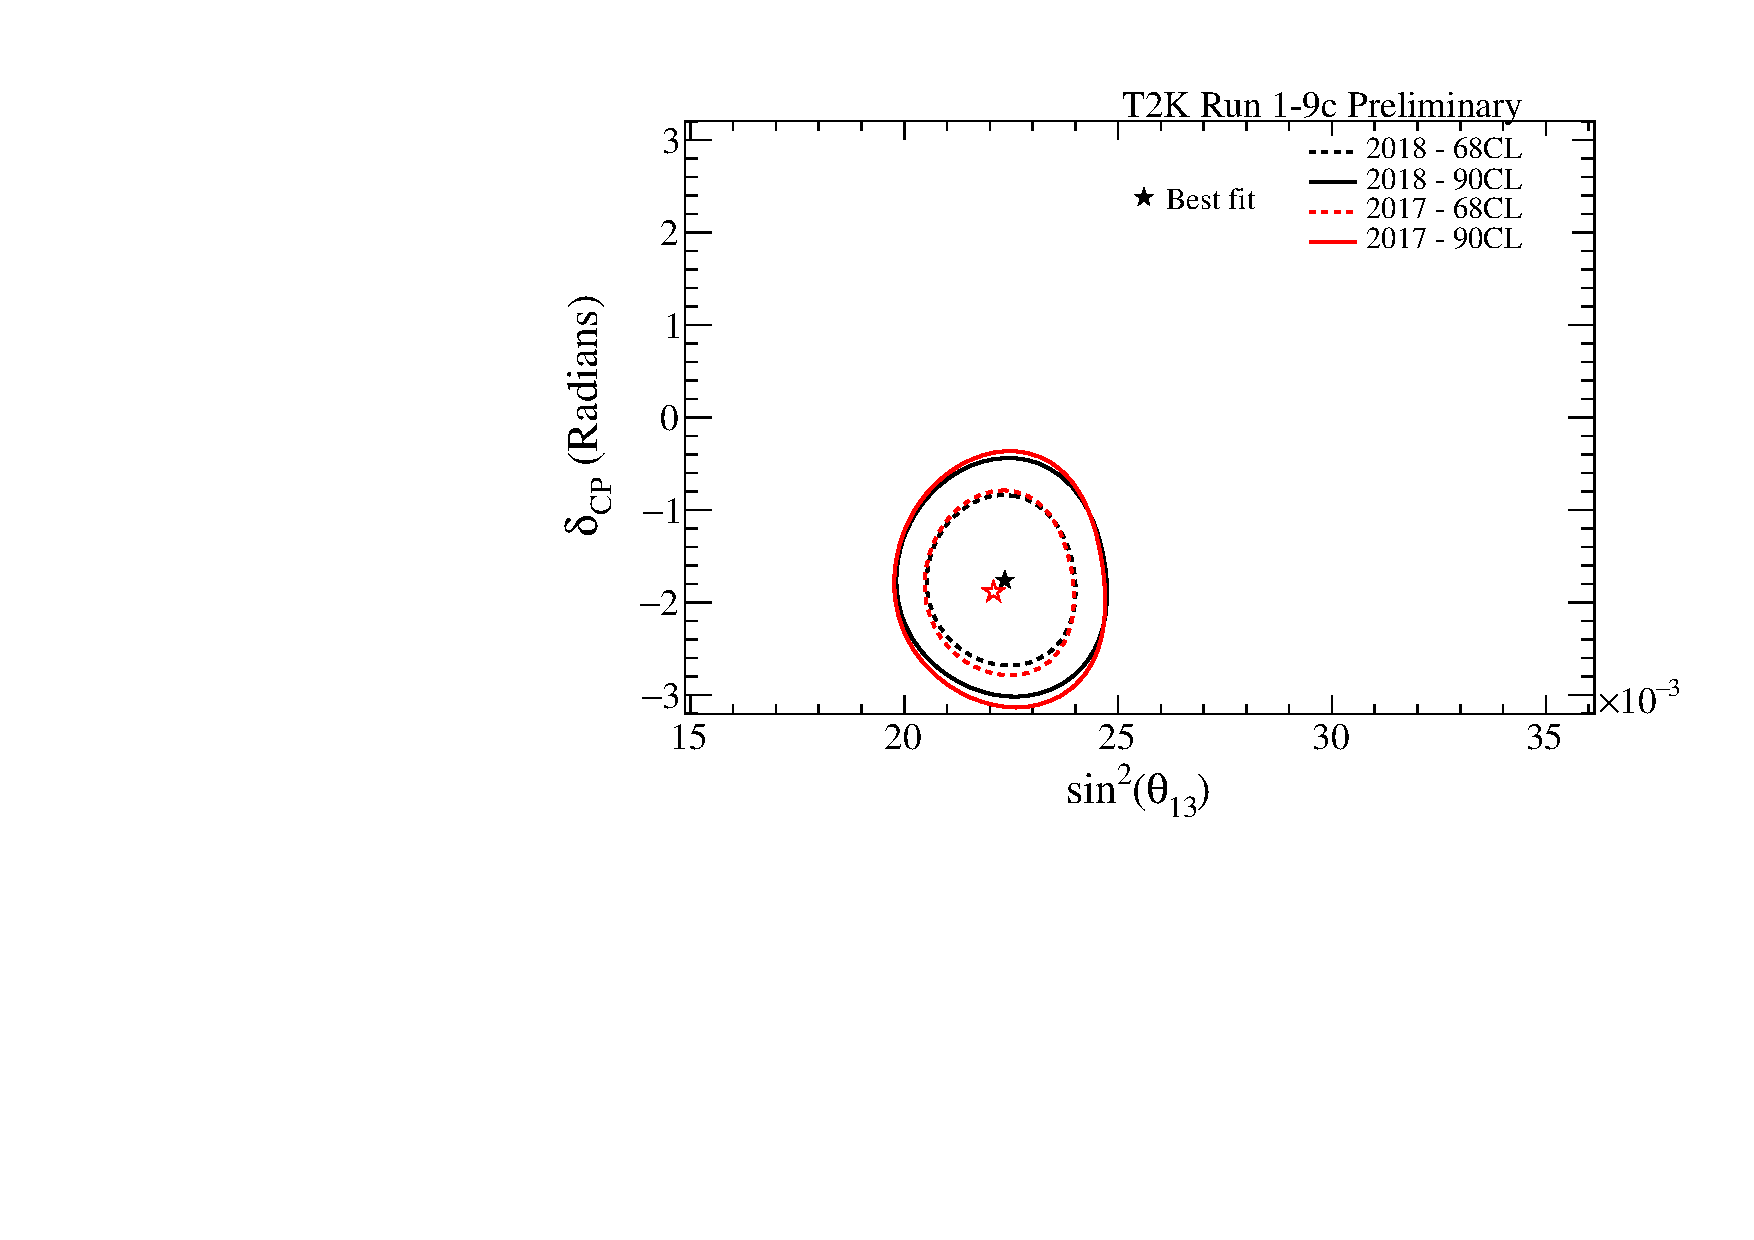
\includegraphics[width=0.9\textwidth]{images/data/comparison/appearance_wrc_normal_2018_v_2017}
		\caption{\appearance NH with reactor constraint}
	\end{subfigure}
	\begin{subfigure}[b]{0.49\textwidth}
		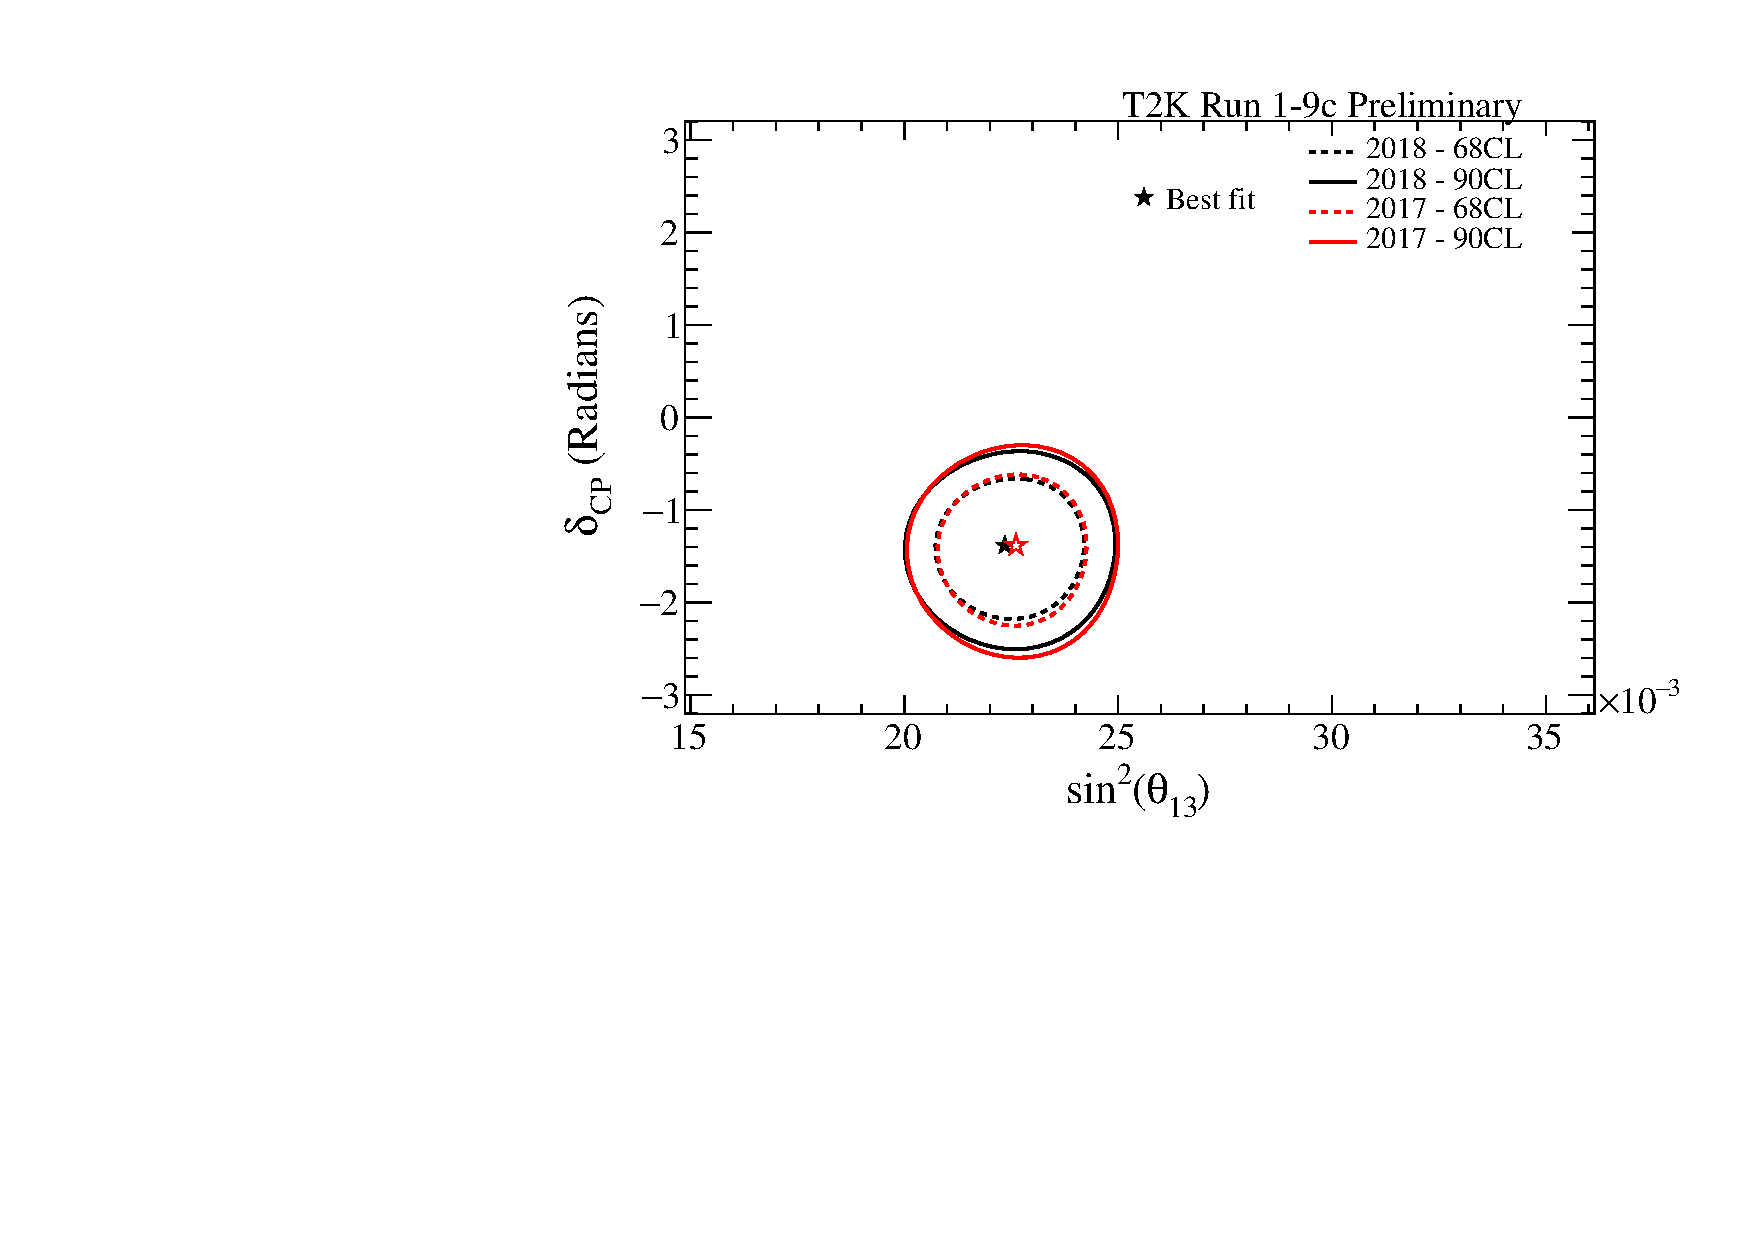
\includegraphics[width=0.9\textwidth]{images/data/comparison/appearance_wrc_inverted_2018_v_2017}
		\caption{\appearance IH with reactor constraint}
	\end{subfigure}
	\begin{subfigure}[b]{0.49\textwidth}
		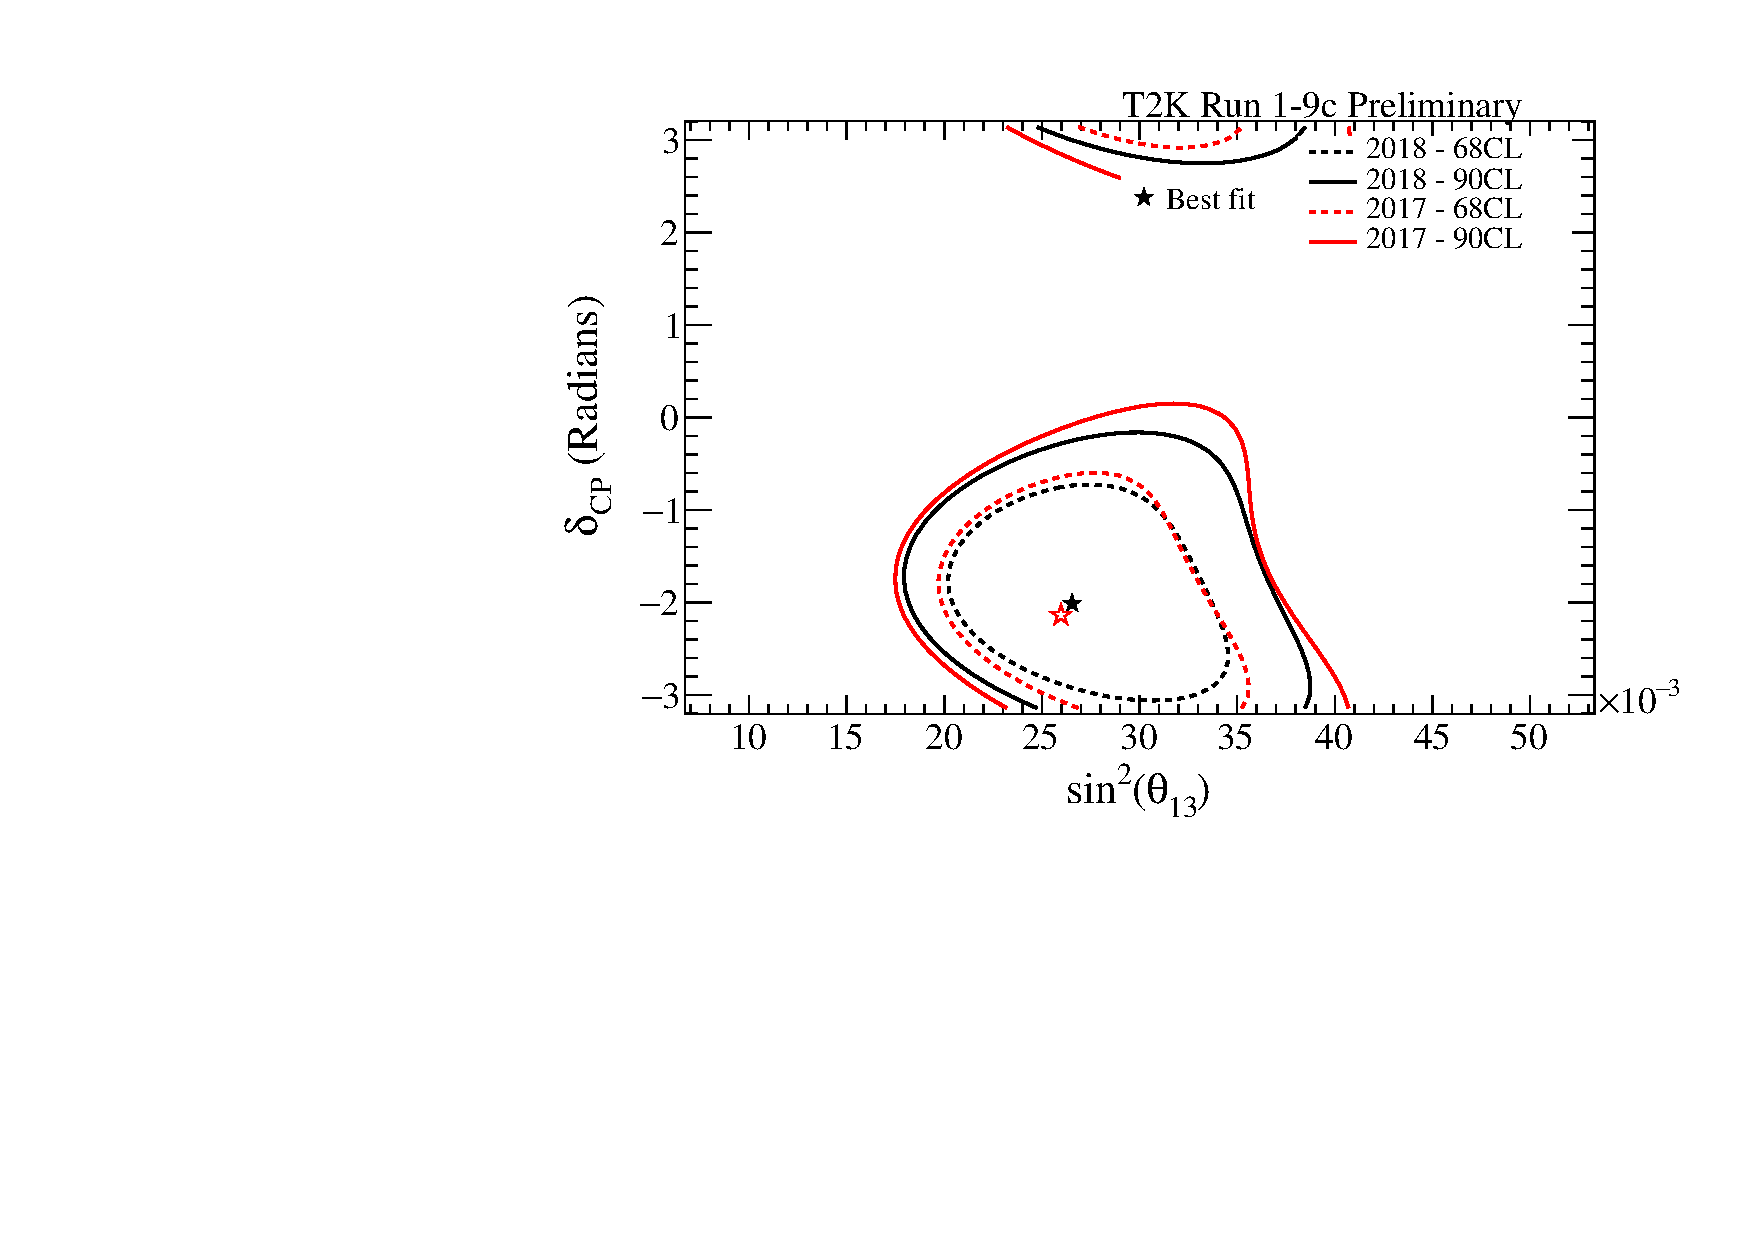
\includegraphics[width=0.9\textwidth]{images/data/comparison/appearance_worc_normal_2018_v_2017}
		\caption{\appearance NH without reactor constraint}
	\end{subfigure}
	\begin{subfigure}[b]{0.49\textwidth}
		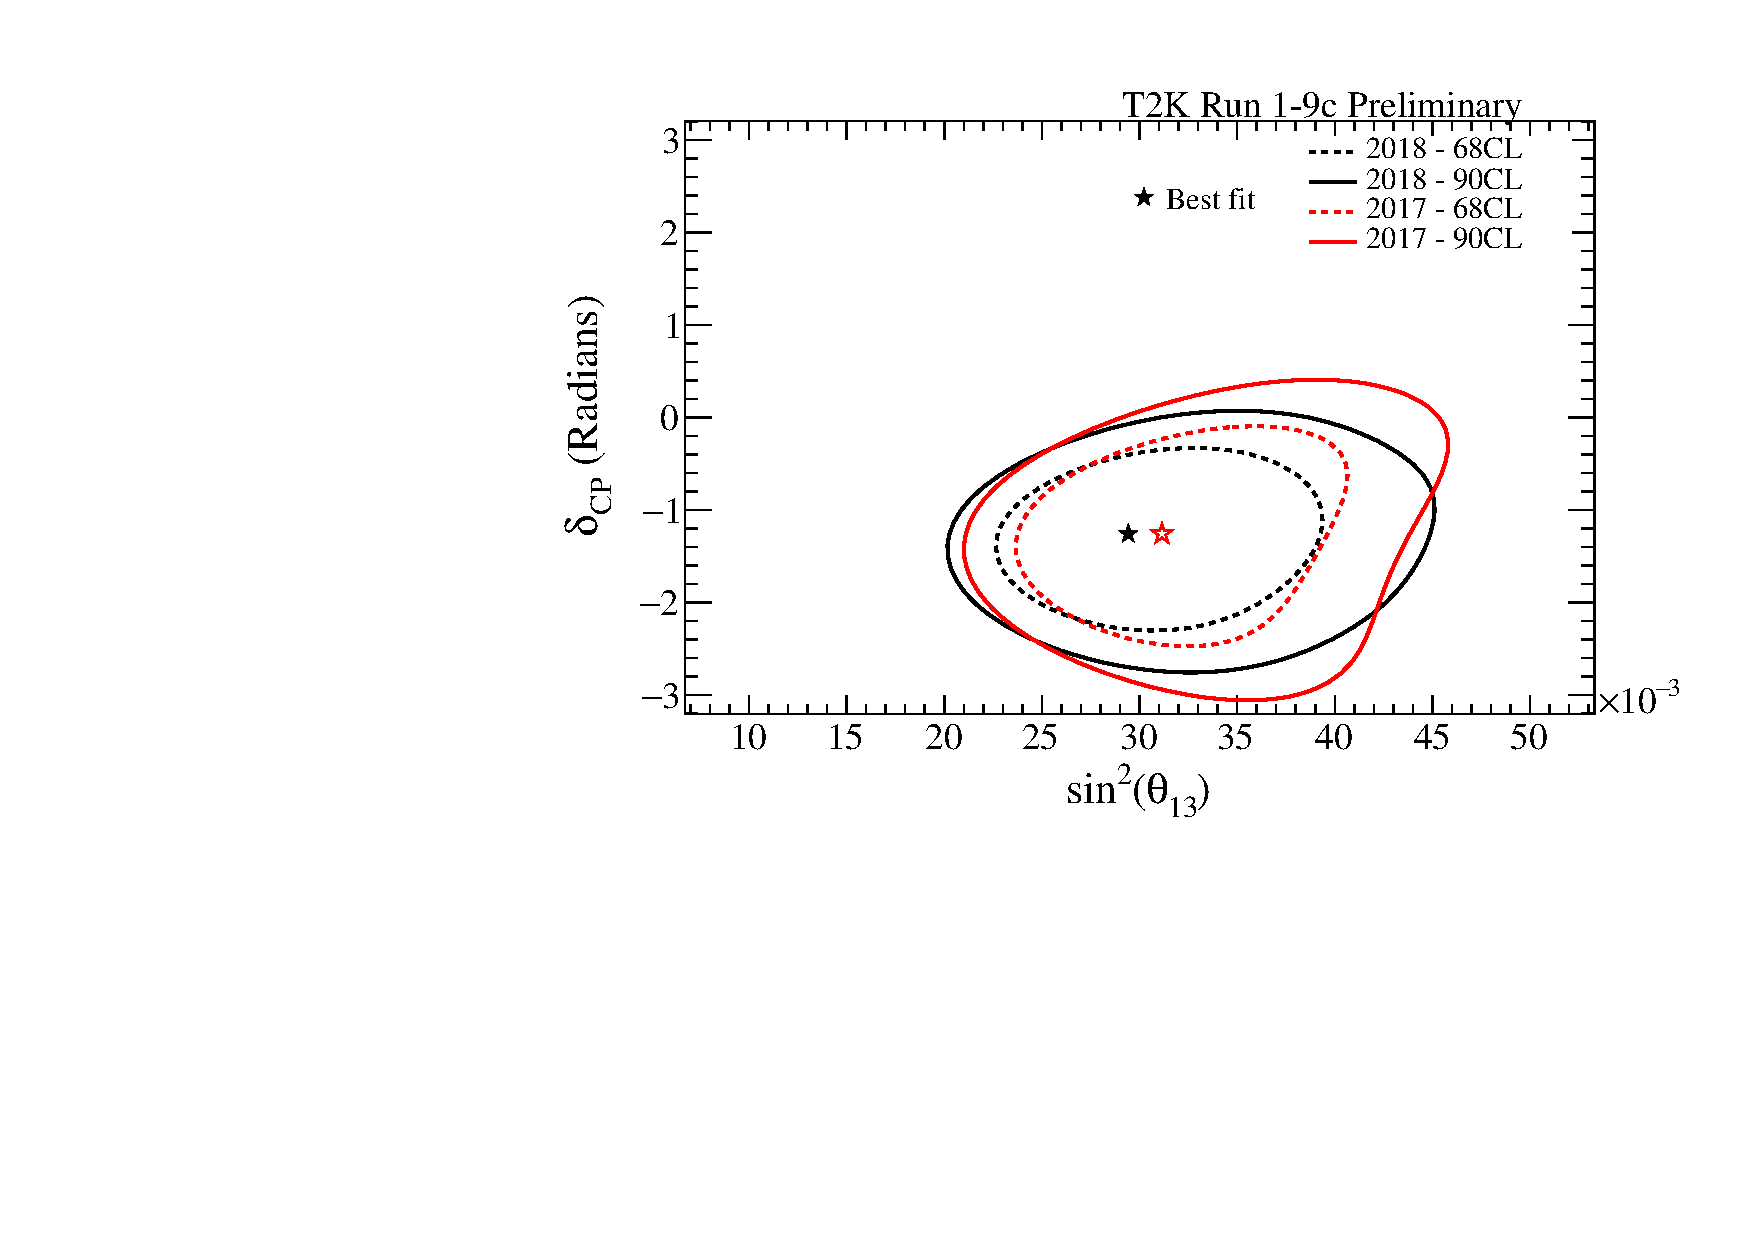
\includegraphics[width=0.9\textwidth]{images/data/comparison/appearance_worc_inverted_2018_v_2017}
		\caption{\appearance IH without reactor constraint}
	\end{subfigure}
	\caption {
		Contours at 68\% and 90\% CL for \appearance with and without reactor constraint. Normal and inverted hierarchy contours are independent. All 5 samples were used to produce these fits.
	}
	\label{fig:ssqth13_vs_dcp_data_compare}
\end{figure*}
\clearpage

\subsection{Results for \disappearance}

The result for \disappearance with reactor constraint and T2K only is shown in fig.~\ref{fig:ssqth23_vs_dmsq_data_compare}. The notable changes in the disappearance fits are a shift of the contour towards lower values of \dmsq (for both normal and inverted hierarchy), a move away from maximal disappearance and a broadening of the contour in the \ssqthtwothree dimension.

\begin{figure*}[htb]
	\center
	\begin{subfigure}[b]{0.49\textwidth}
		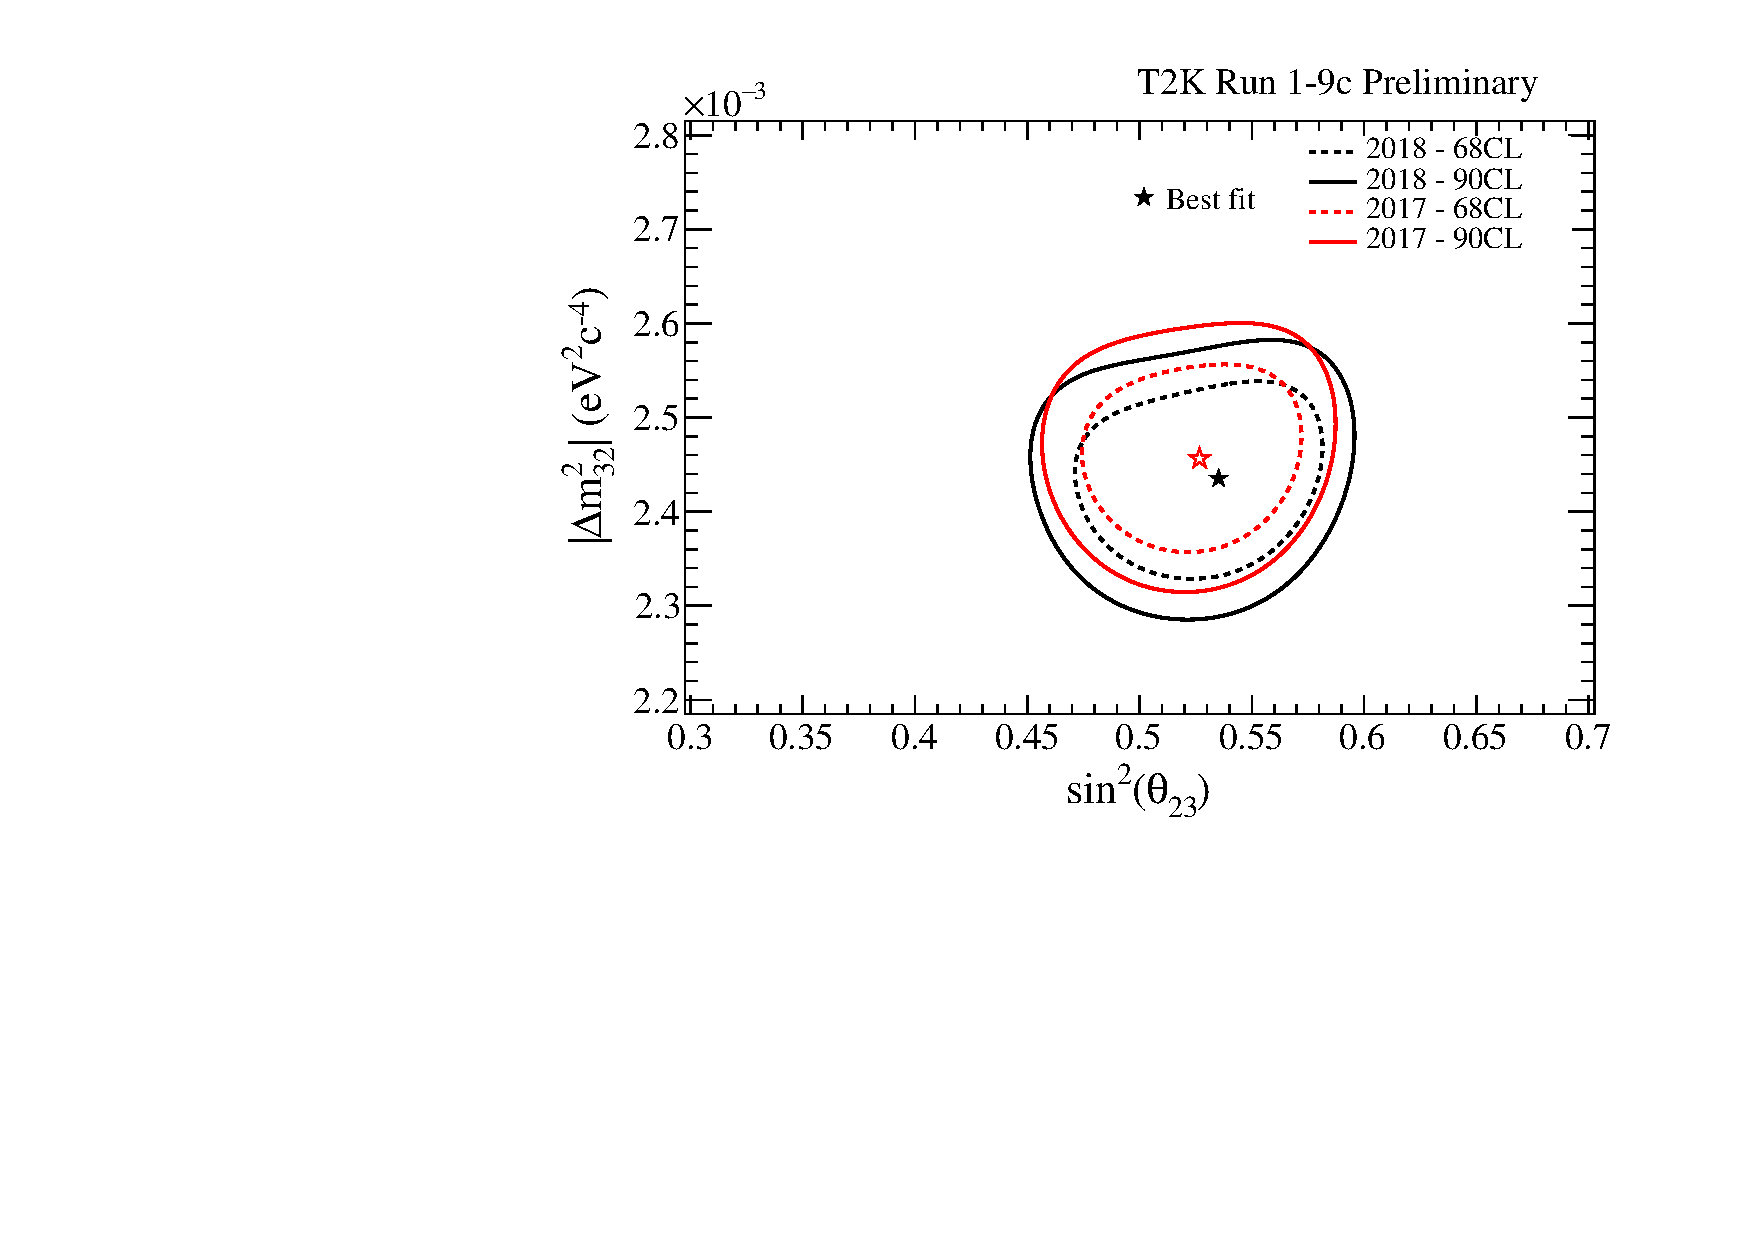
\includegraphics[width=0.9\textwidth]{images/data/comparison/disappearance_wrc_normal_2018_v_2017}
		\caption{\disappearance NH with reactor constraint}
	\end{subfigure}
	\begin{subfigure}[b]{0.49\textwidth}
		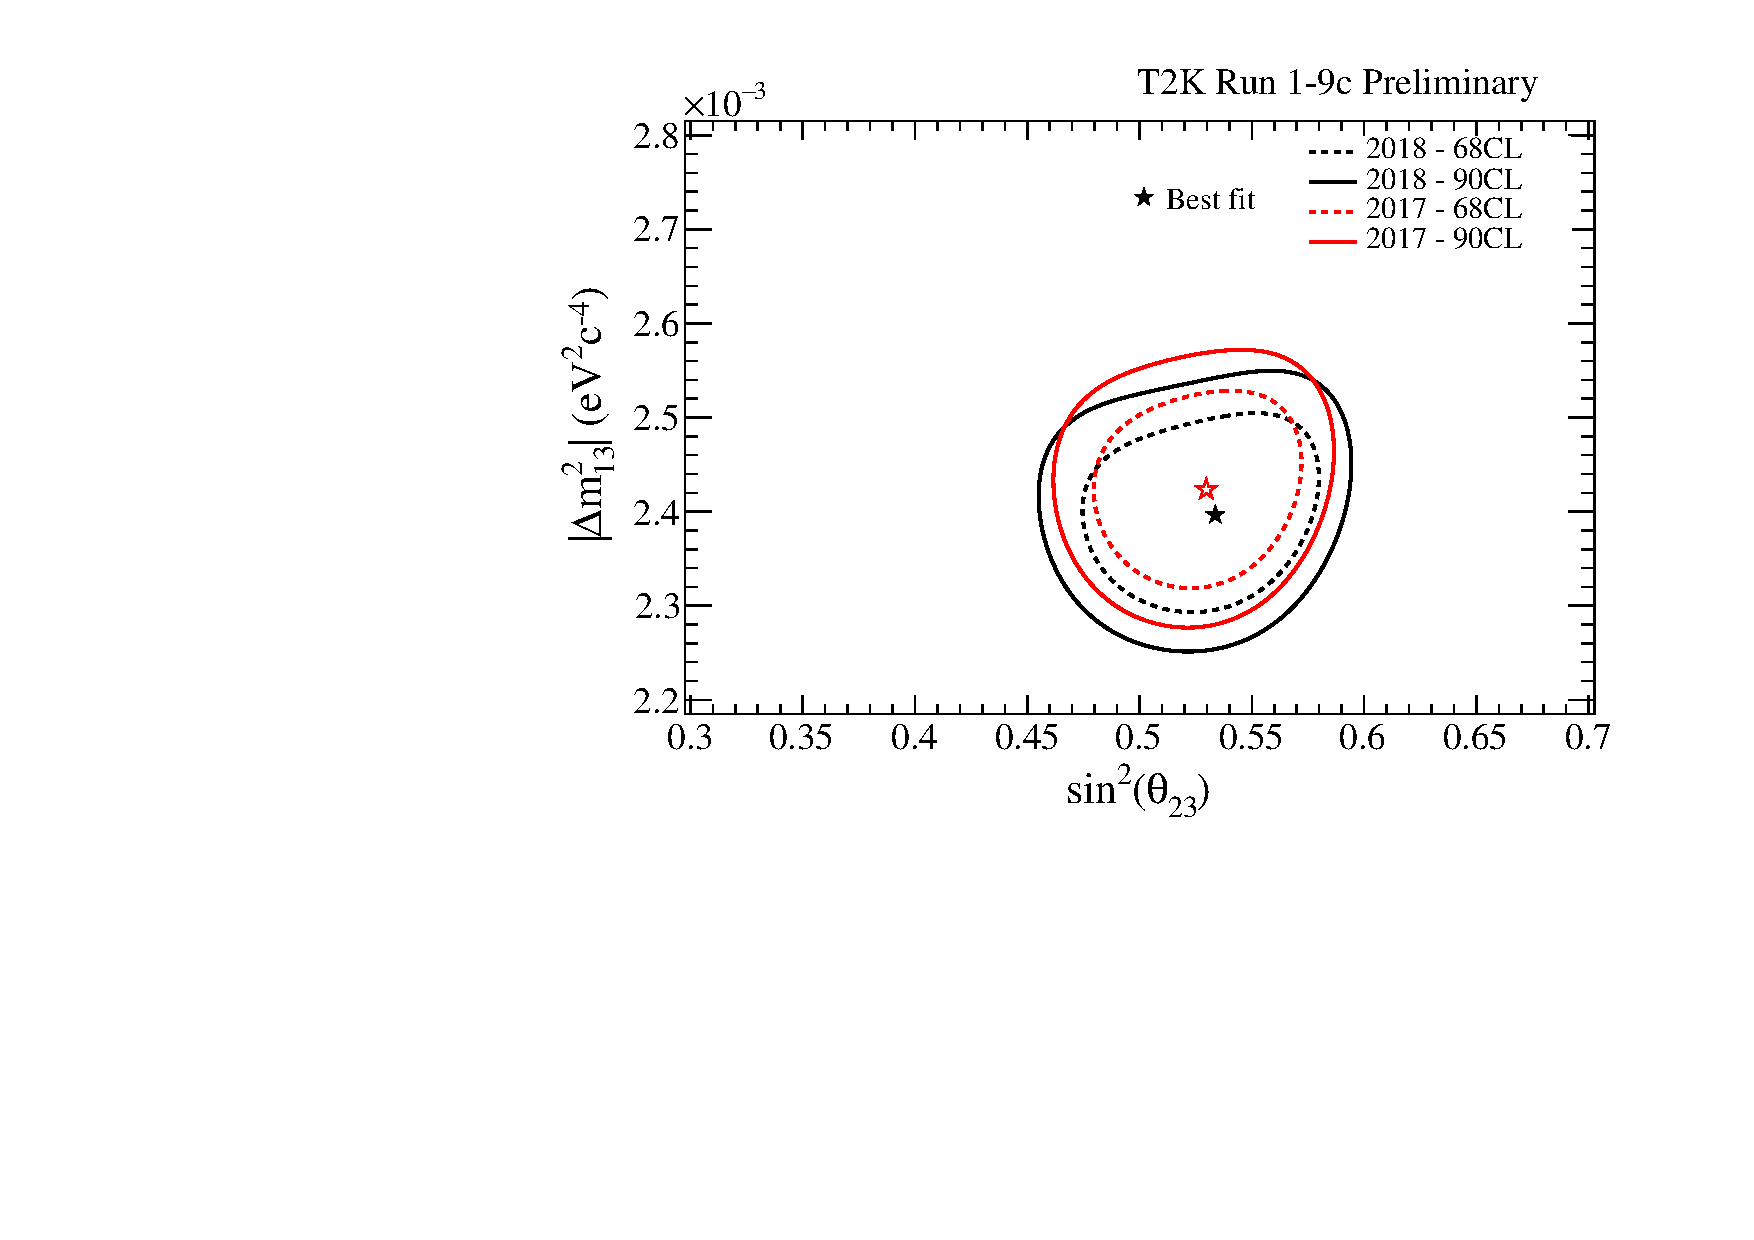
\includegraphics[width=0.9\textwidth]{images/data/comparison/disappearance_wrc_inverted_2018_v_2017}
		\caption{\disappearance IH with reactor constraint}
	\end{subfigure}
	\begin{subfigure}[b]{0.49\textwidth}
		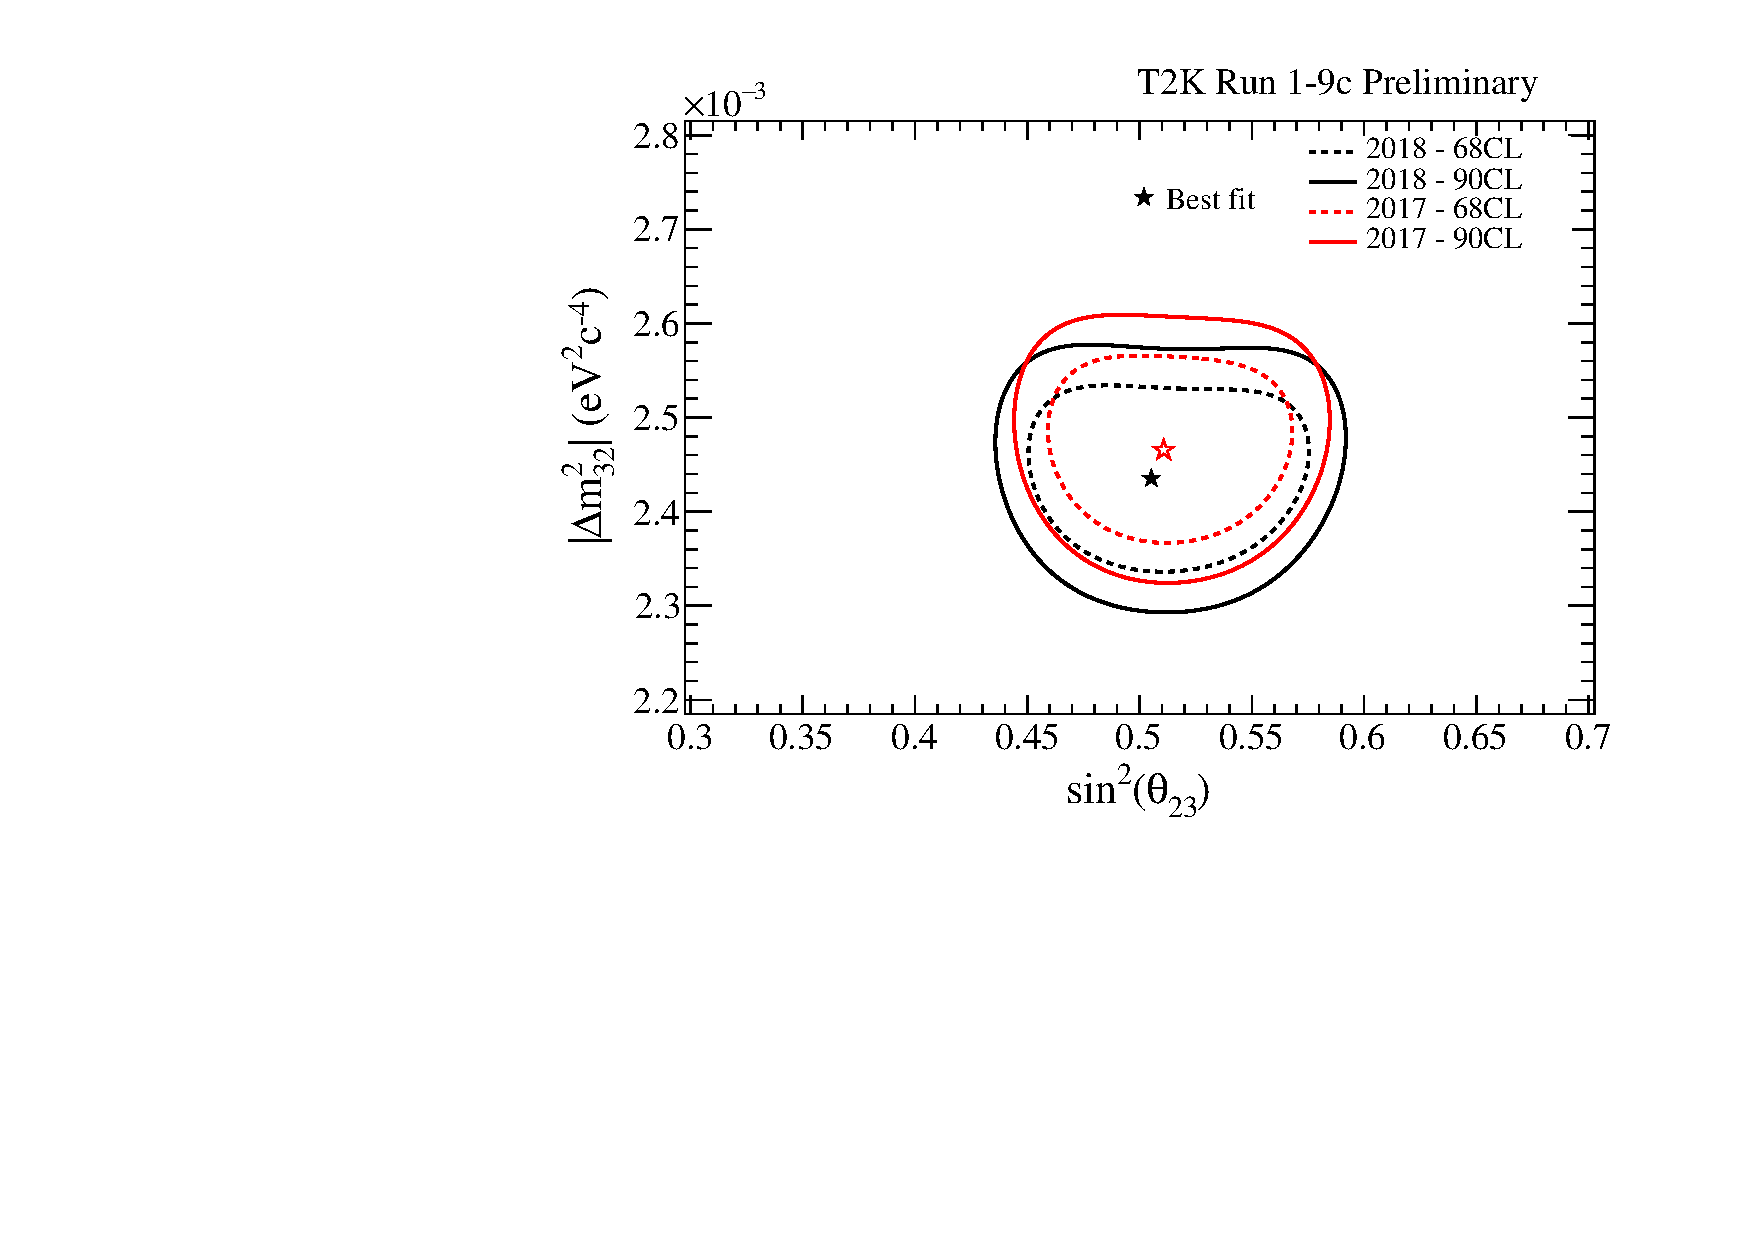
\includegraphics[width=0.9\textwidth]{images/data/comparison/disappearance_worc_normal_2018_v_2017}
		\caption{\disappearance NH without reactor constraint}
	\end{subfigure}
	\begin{subfigure}[b]{0.49\textwidth}
		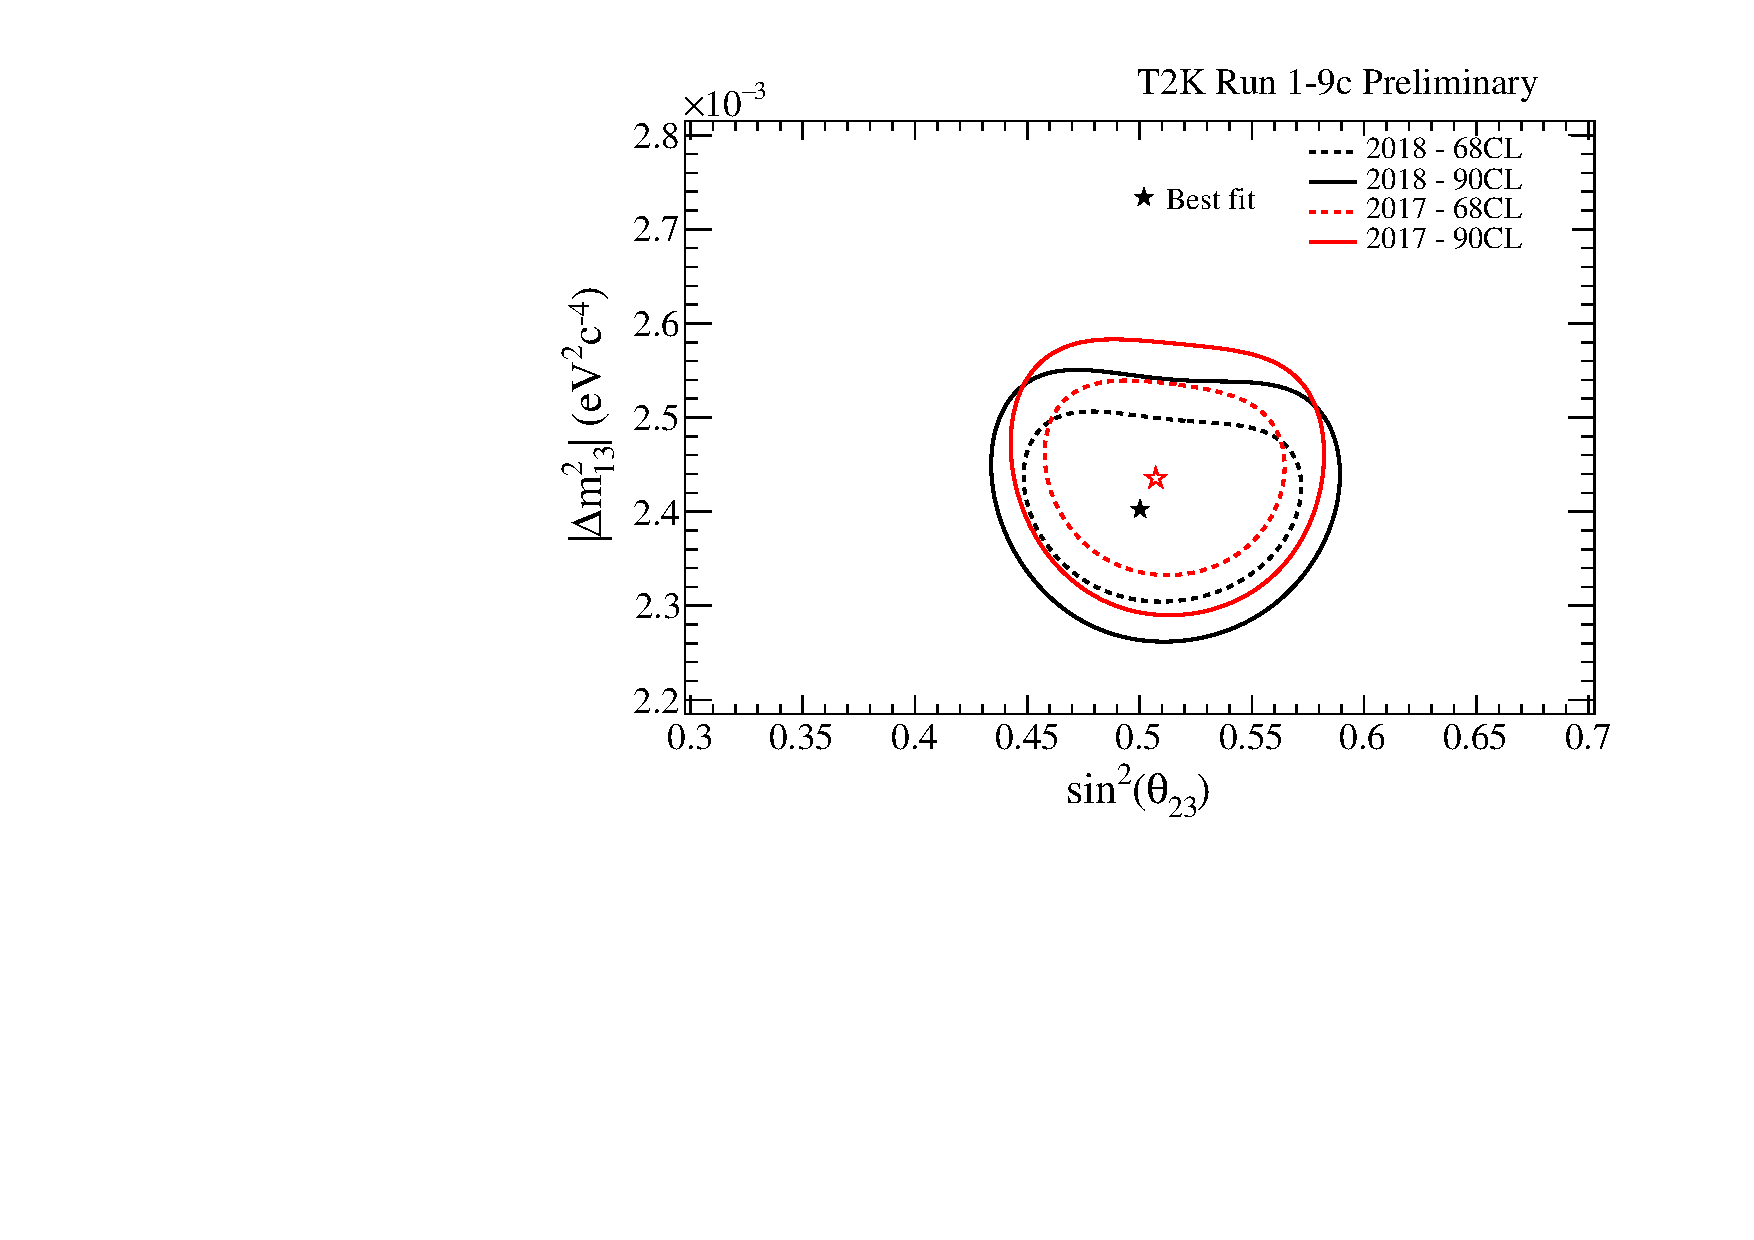
\includegraphics[width=0.9\textwidth]{images/data/comparison/disappearance_worc_inverted_2018_v_2017}
		\caption{\disappearance IH without reactor constraint}
	\end{subfigure}
	\caption {
		Contours at 68\% and 90\% CL for \disappearance with and without reactor constraint. Normal and inverted hierarchy contours are independent. All 5 samples were used to produce these fits.
	}
	\label{fig:ssqth23_vs_dmsq_data_compare}
\end{figure*}

In \PrevRunPeriod, the data contour is both narrower and shifted with respect to the prediction of the best-fit Asimov (\cref{fig:disappearance_check}), whereas the \RunPeriod data contour shows better agreement with the best-fit prediction, though remaining somewhat narrower. The corresponding RHC one-ring $\mu$-like observed and best-fit spectra are also shown. Therefore, the broadening of the contour in \RunPeriod can be explained as the result of a shift towards a more PMNS-like result.

\begin{figure*}[htb]
	\center
	\begin{subfigure}[b]{0.49\textwidth}
		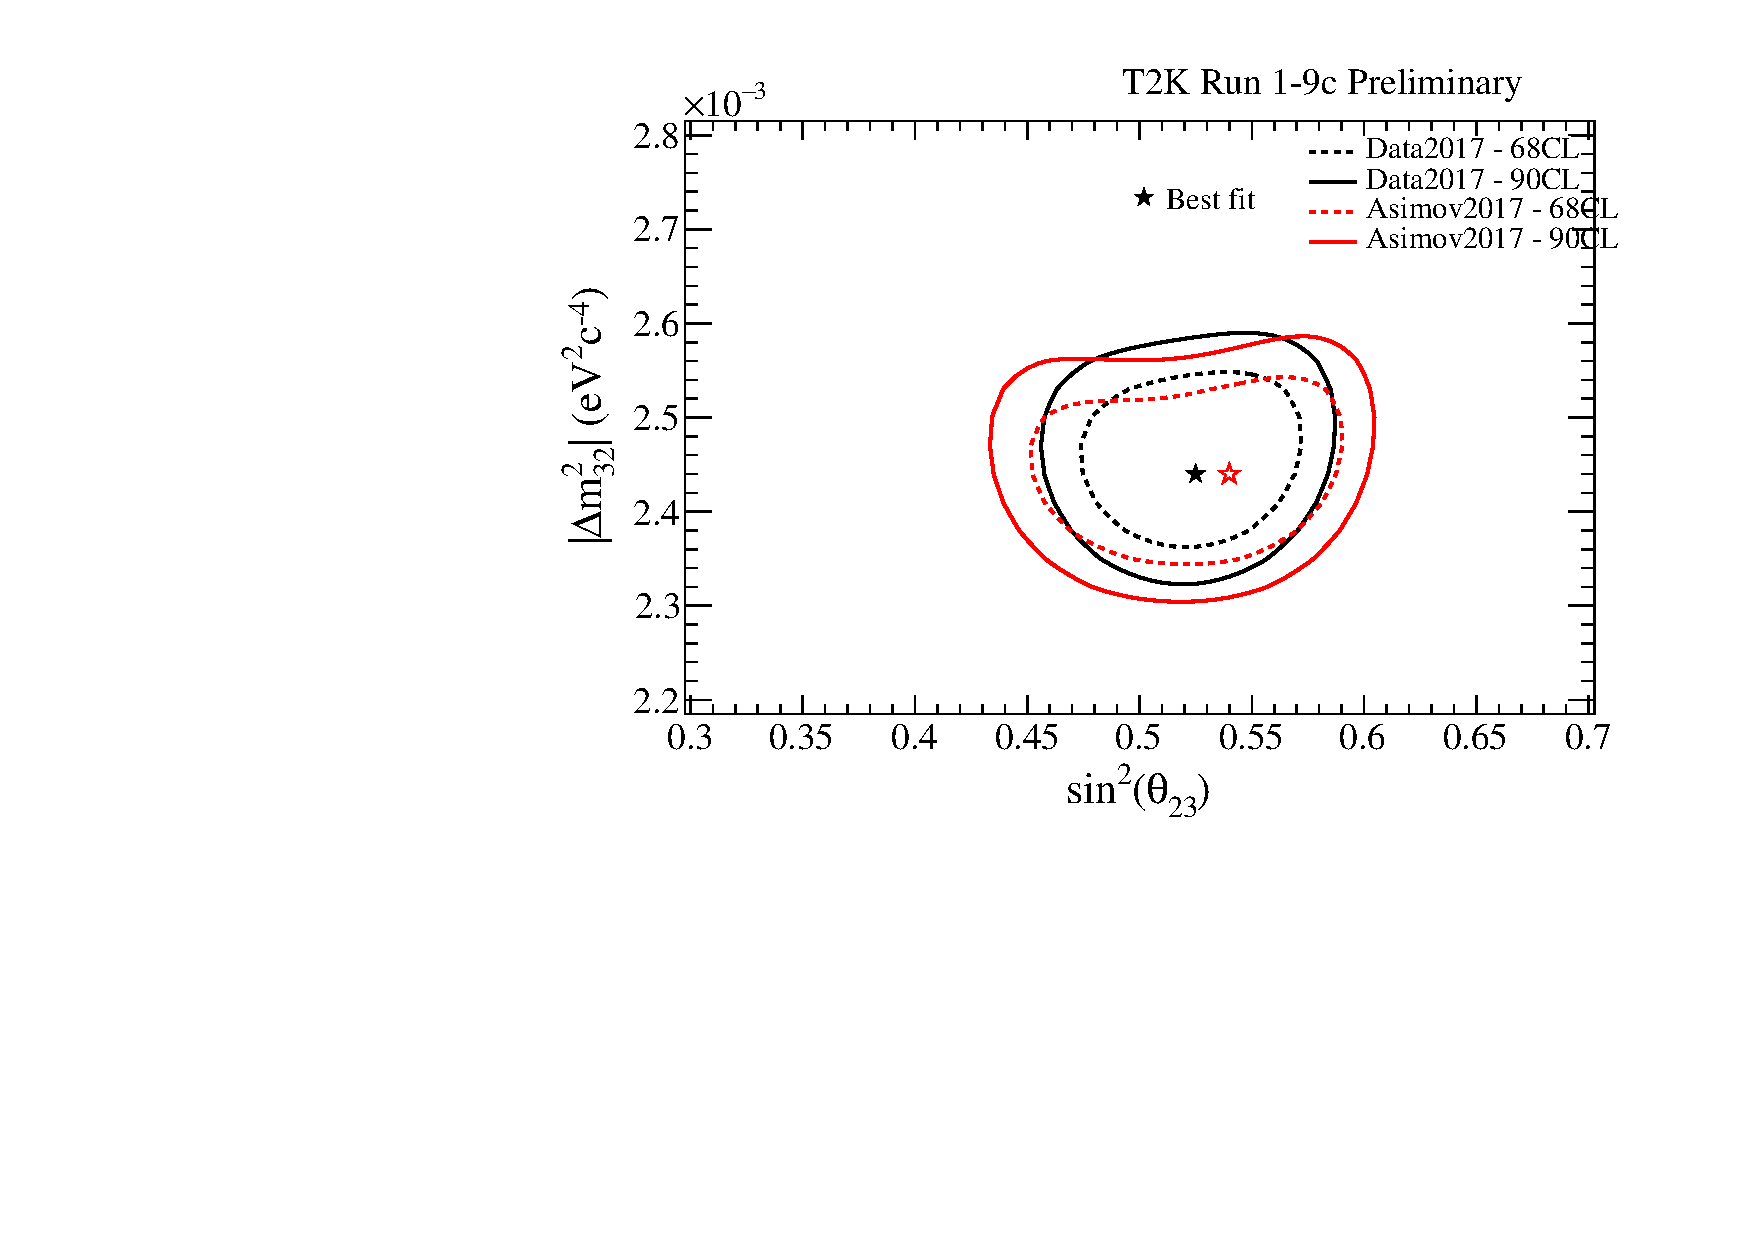
\includegraphics[width=0.9\textwidth]{images/checks/disappearance/Data2017_v_Asimov2017}
		\caption{\PrevRunPeriod}
	\end{subfigure}
	\begin{subfigure}[b]{0.49\textwidth}
		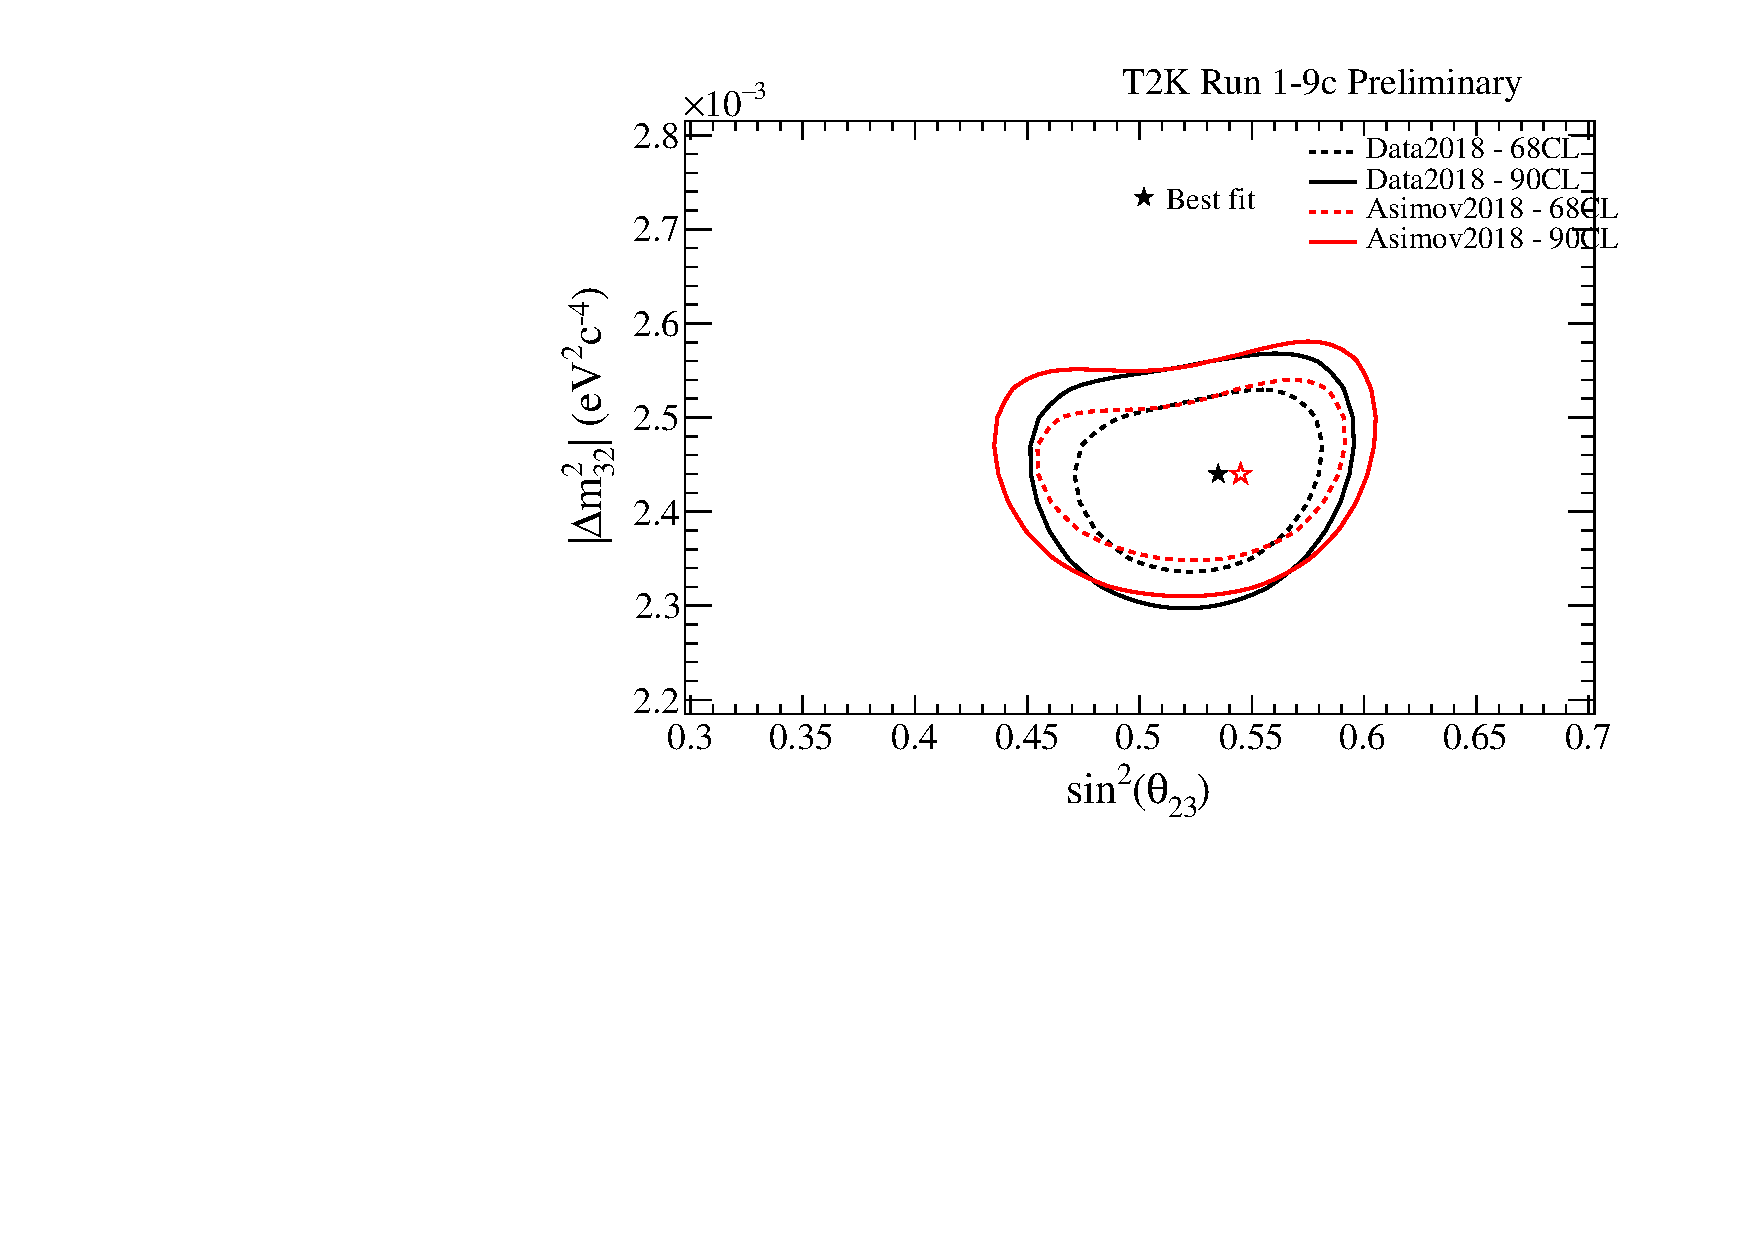
\includegraphics[width=0.9\textwidth]{images/checks/disappearance/Data2018_v_Asimov2018}
		\caption{\RunPeriod}
	\end{subfigure}
	
	\begin{subfigure}[b]{0.49\textwidth}
		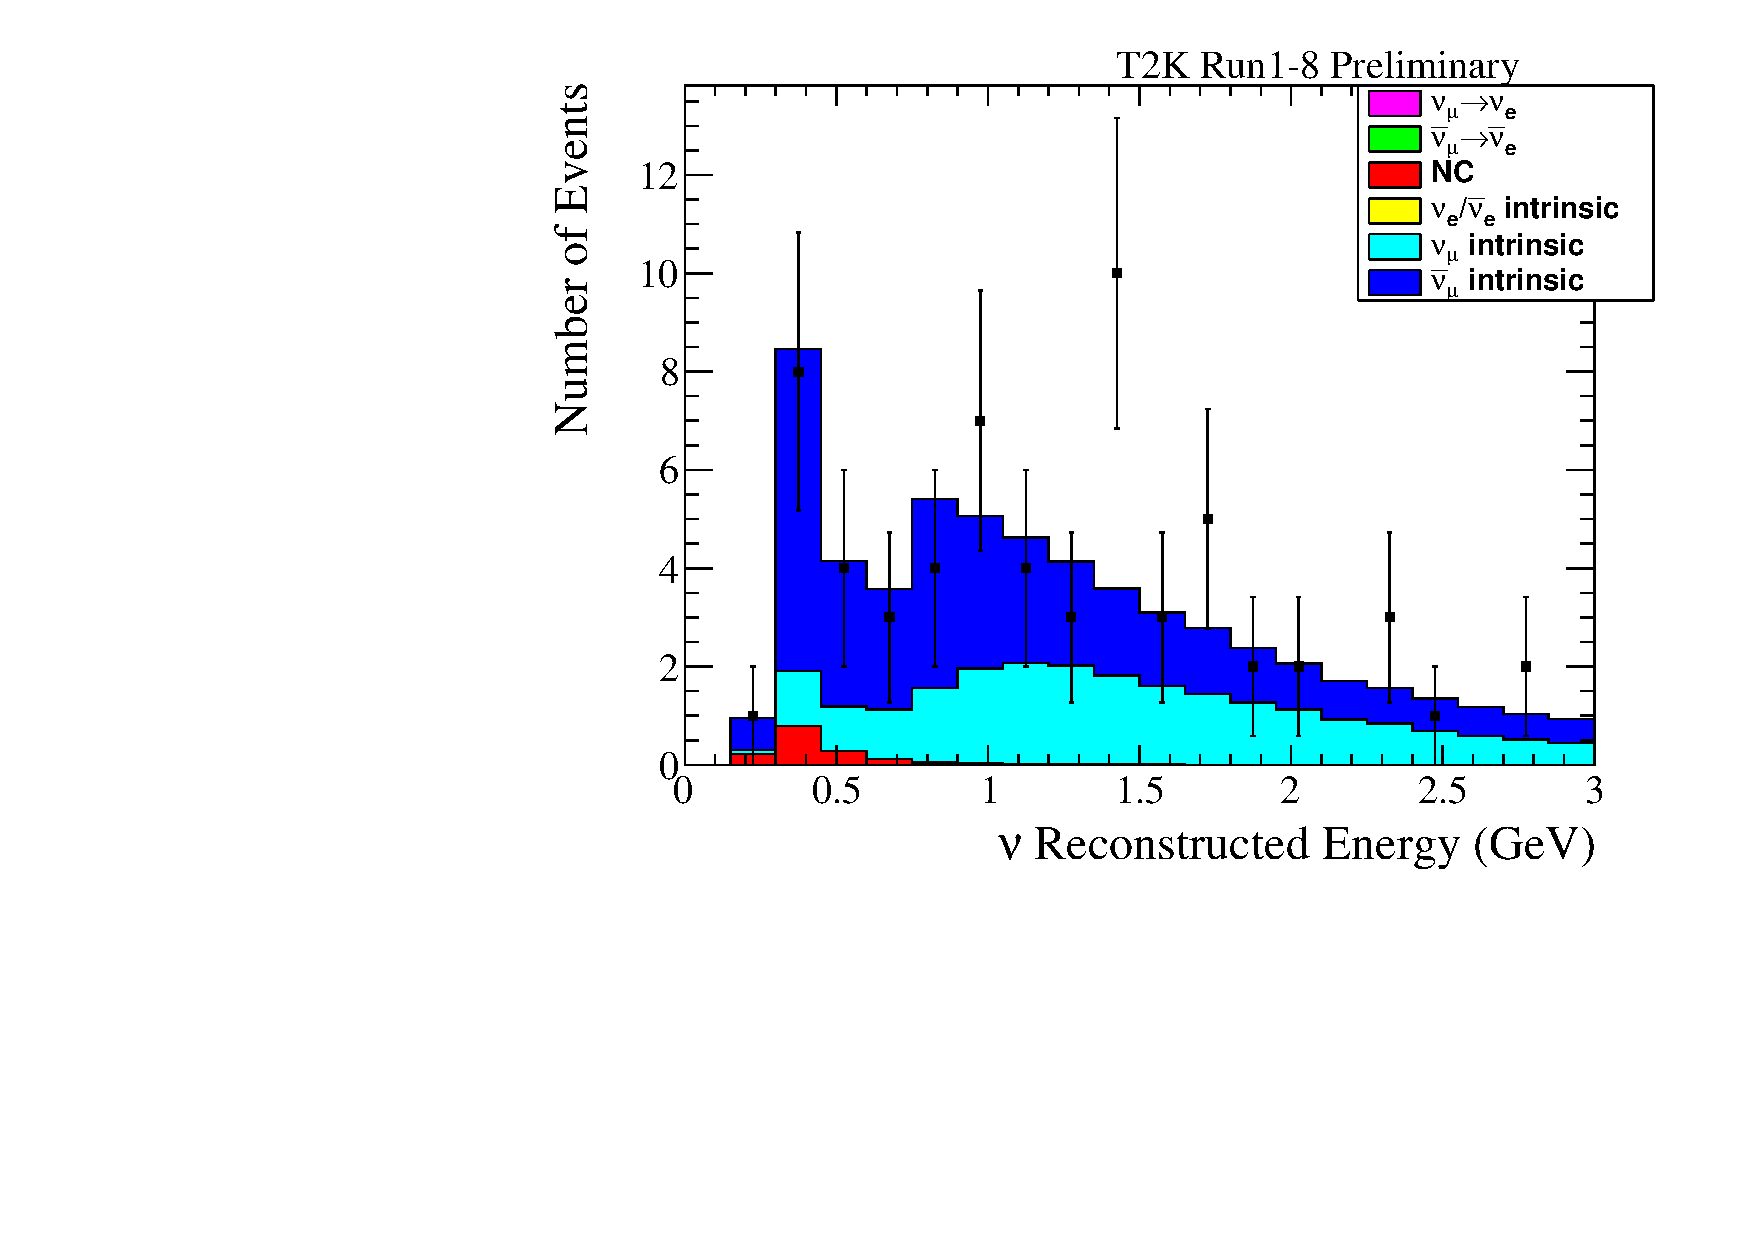
\includegraphics[width=0.9\textwidth]{images/checks/disappearance/spectrum_asimov2017_RHC1Rmu_data}
		\caption{\PrevRunPeriod RHC one-ring $\mu$-like spectra}
	\end{subfigure}
	\begin{subfigure}[b]{0.49\textwidth}
		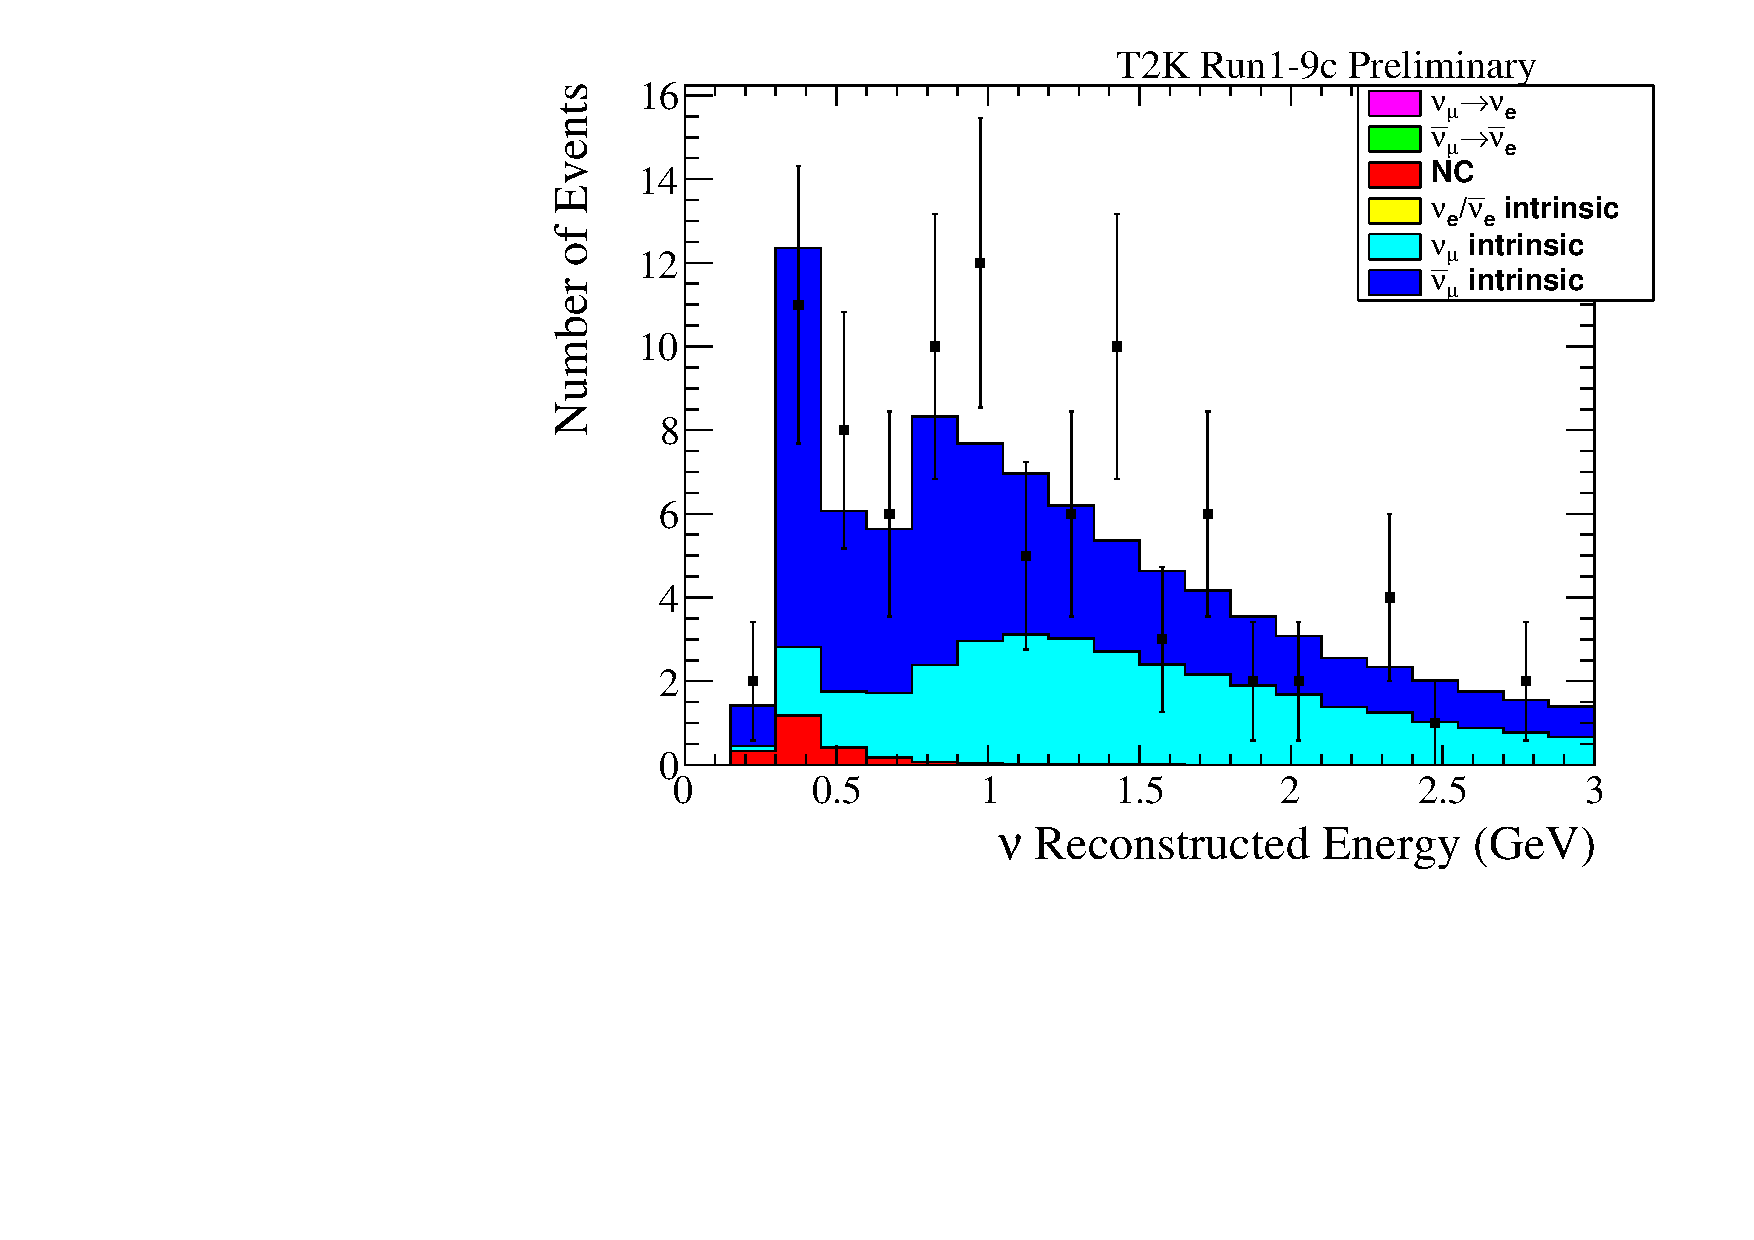
\includegraphics[width=0.9\textwidth]{images/checks/disappearance/spectrum_asimov2018_RHC1Rmu_data}
		\caption{\RunPeriod RHC one-ring $\mu$-like spectra}
	\end{subfigure}
	\caption {
		The top row shows normal hierarchy contours at 68\% and 90\% CL for \disappearance with the reactor constraint compared to a fit of the best-fit Asimov corresponding to the stated run period. No smearing is applied. The bottom row shows the observed and predicted spectrum from \PrevRunPeriod and \RunPeriod.
	}
	\label{fig:disappearance_check}
\end{figure*}

\iffalse
A potential explanation for the broadening of the contour, despite the increase in statistics could come from a shift in the value of \ssqthtwothree away from maximal disappearance ($\sin^2\theta_{23} \simeq 0.51$).
\fi

\clearpage

\subsection{Results for \deltacp}

The result for \deltacp with reactor constraint and T2K only is shown in fig.~\ref{fig:dcp_data_compare}. The best-fit points are little changed relative to \PrevRunPeriod, though a stronger constraint is evident, particularly without the reactor constraint applied.

\begin{figure*}[htb]
	\center
	\begin{subfigure}[b]{0.49\textwidth}
		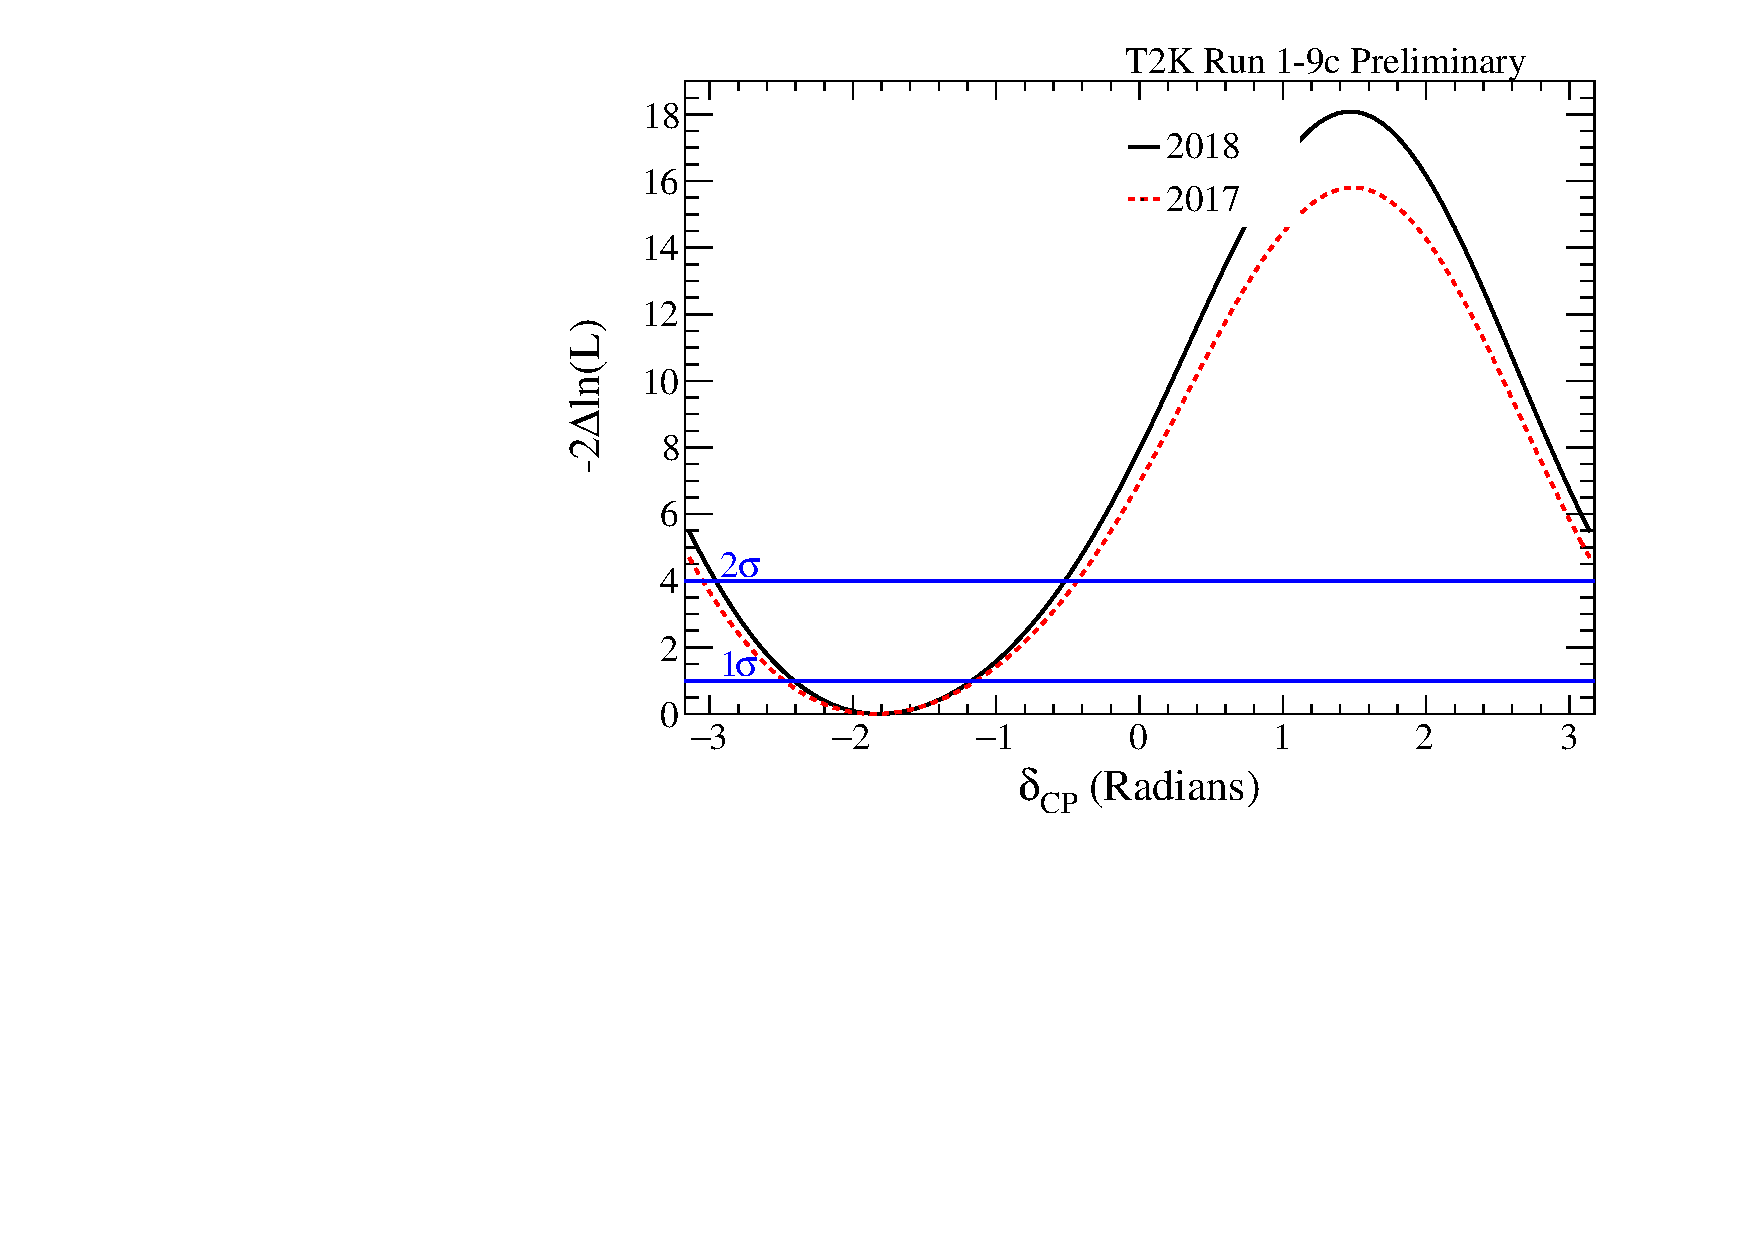
\includegraphics[width=0.9\textwidth]{images/data/comparison/deltacp_wrc_normal_2018_v_2017}
		\caption{\deltacp NH with reactor constraint}
	\end{subfigure}
	\begin{subfigure}[b]{0.49\textwidth}
		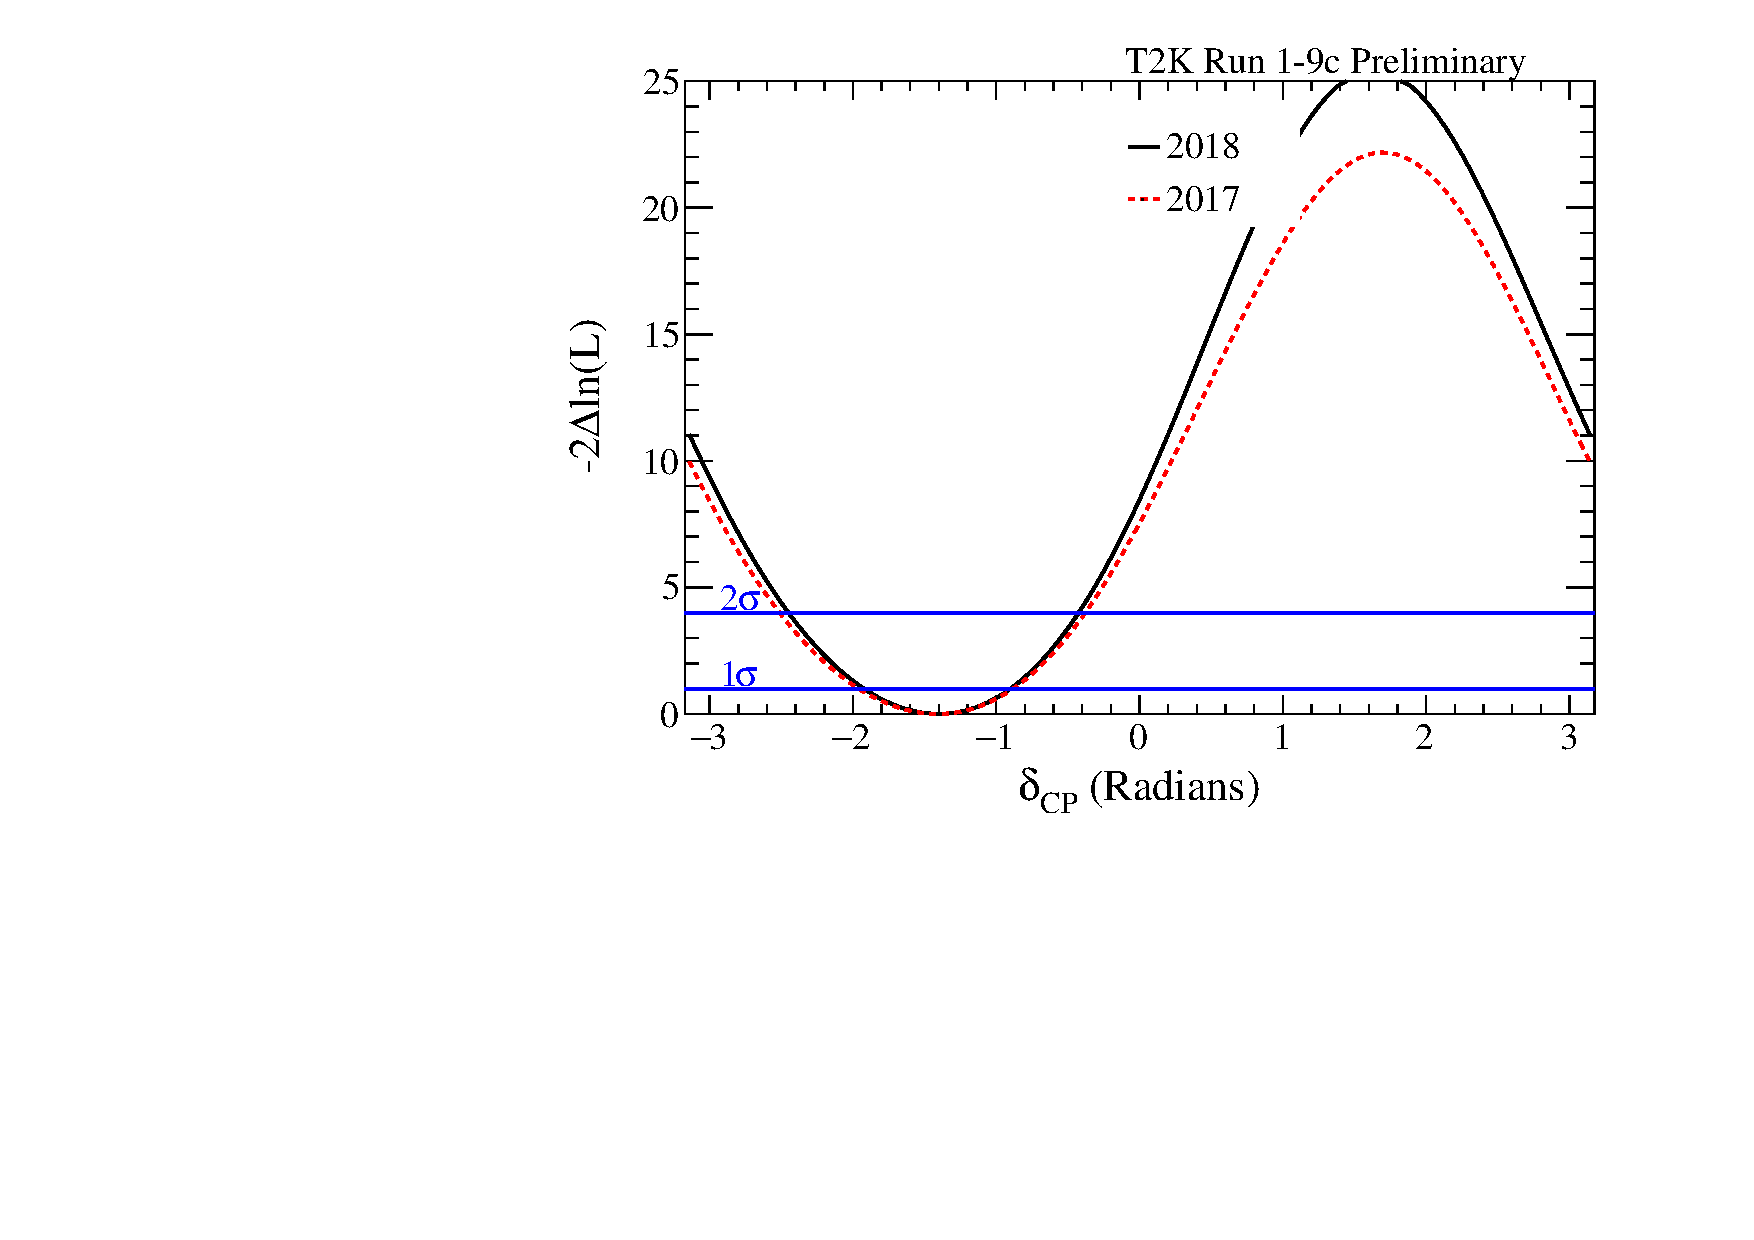
\includegraphics[width=0.9\textwidth]{images/data/comparison/deltacp_wrc_inverted_2018_v_2017}
		\caption{\deltacp IH with reactor constraint}
	\end{subfigure}
	\begin{subfigure}[b]{0.49\textwidth}
		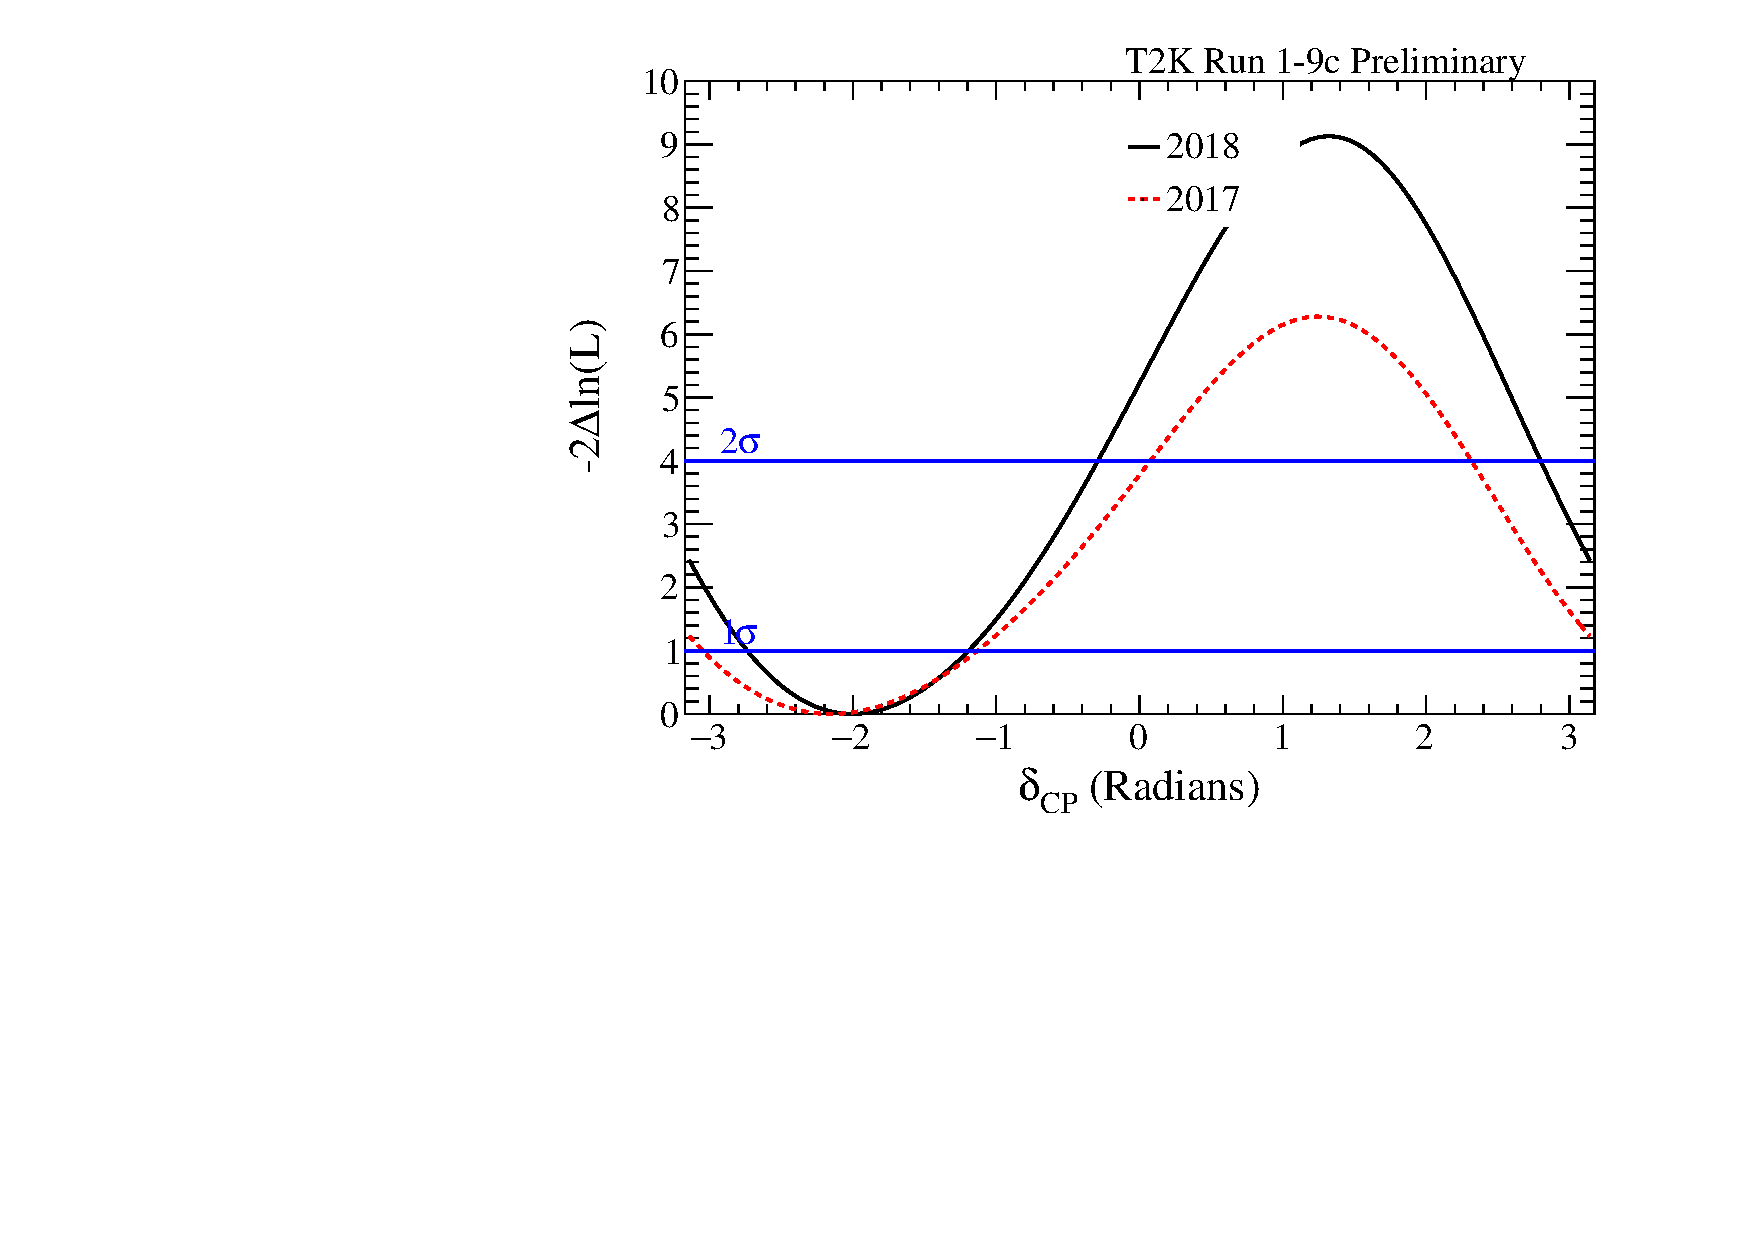
\includegraphics[width=0.9\textwidth]{images/data/comparison/deltacp_worc_normal_2018_v_2017}
		\caption{\deltacp NH without reactor constraint}
	\end{subfigure}
	\begin{subfigure}[b]{0.49\textwidth}
		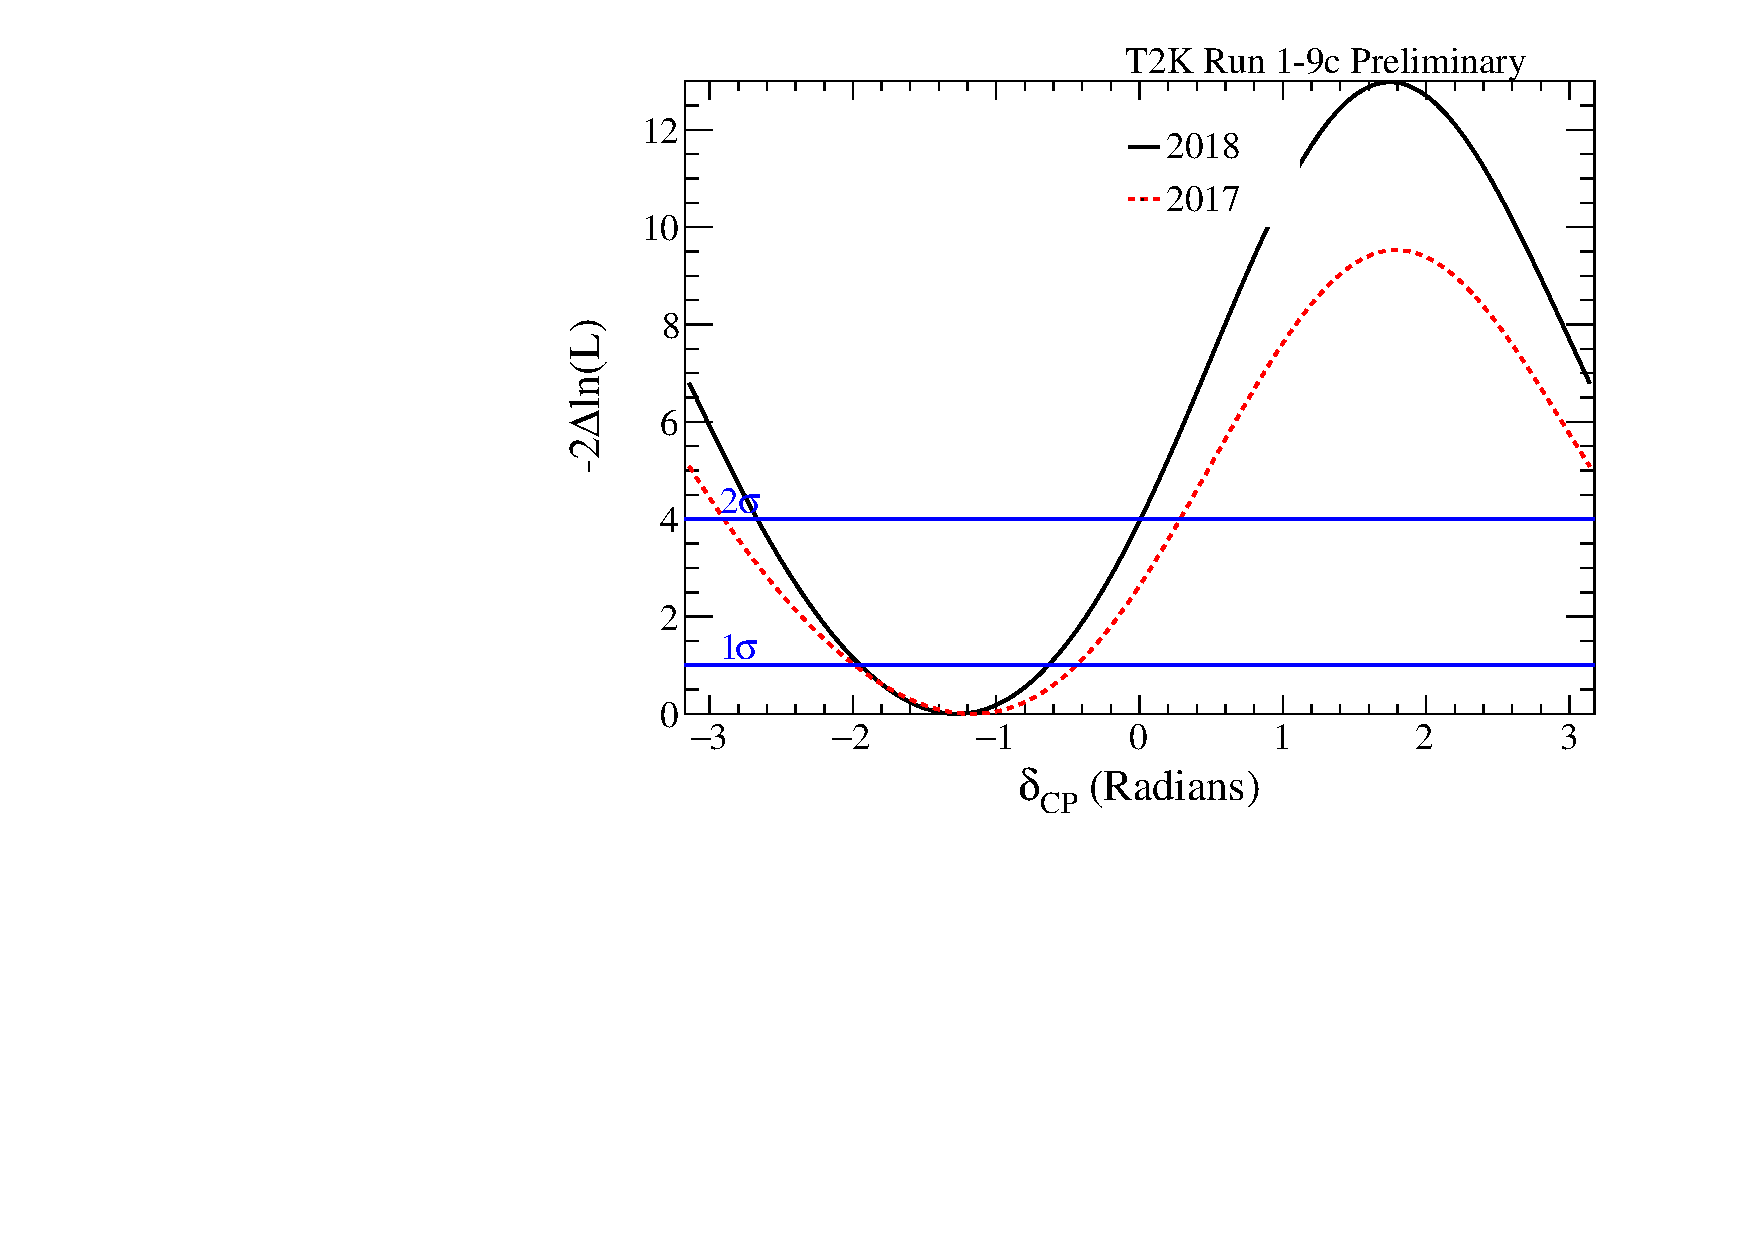
\includegraphics[width=0.9\textwidth]{images/data/comparison/deltacp_worc_inverted_2018_v_2017}
		\caption{\deltacp IH without reactor constraint}
	\end{subfigure}
	\caption {
		The expected $\Delta\chi^2$ distribution as a function of \deltacp with and without reactor constraint. Normal and inverted hierarchy contours are independent. All 5 samples were used to produce these fits.
	}
	\label{fig:dcp_data_compare}
\end{figure*}
\clearpage

\subsection{Results for \ssqthonethree}

The result for \ssqthonethree (without reactor constraint) is shown in fig.~\ref{fig:th13_data_compare}. A small shift in the best-fit value can be observed, along with a tightening of the contour.

\begin{figure*}[htb]
	\center
	\begin{subfigure}[b]{0.49\textwidth}
		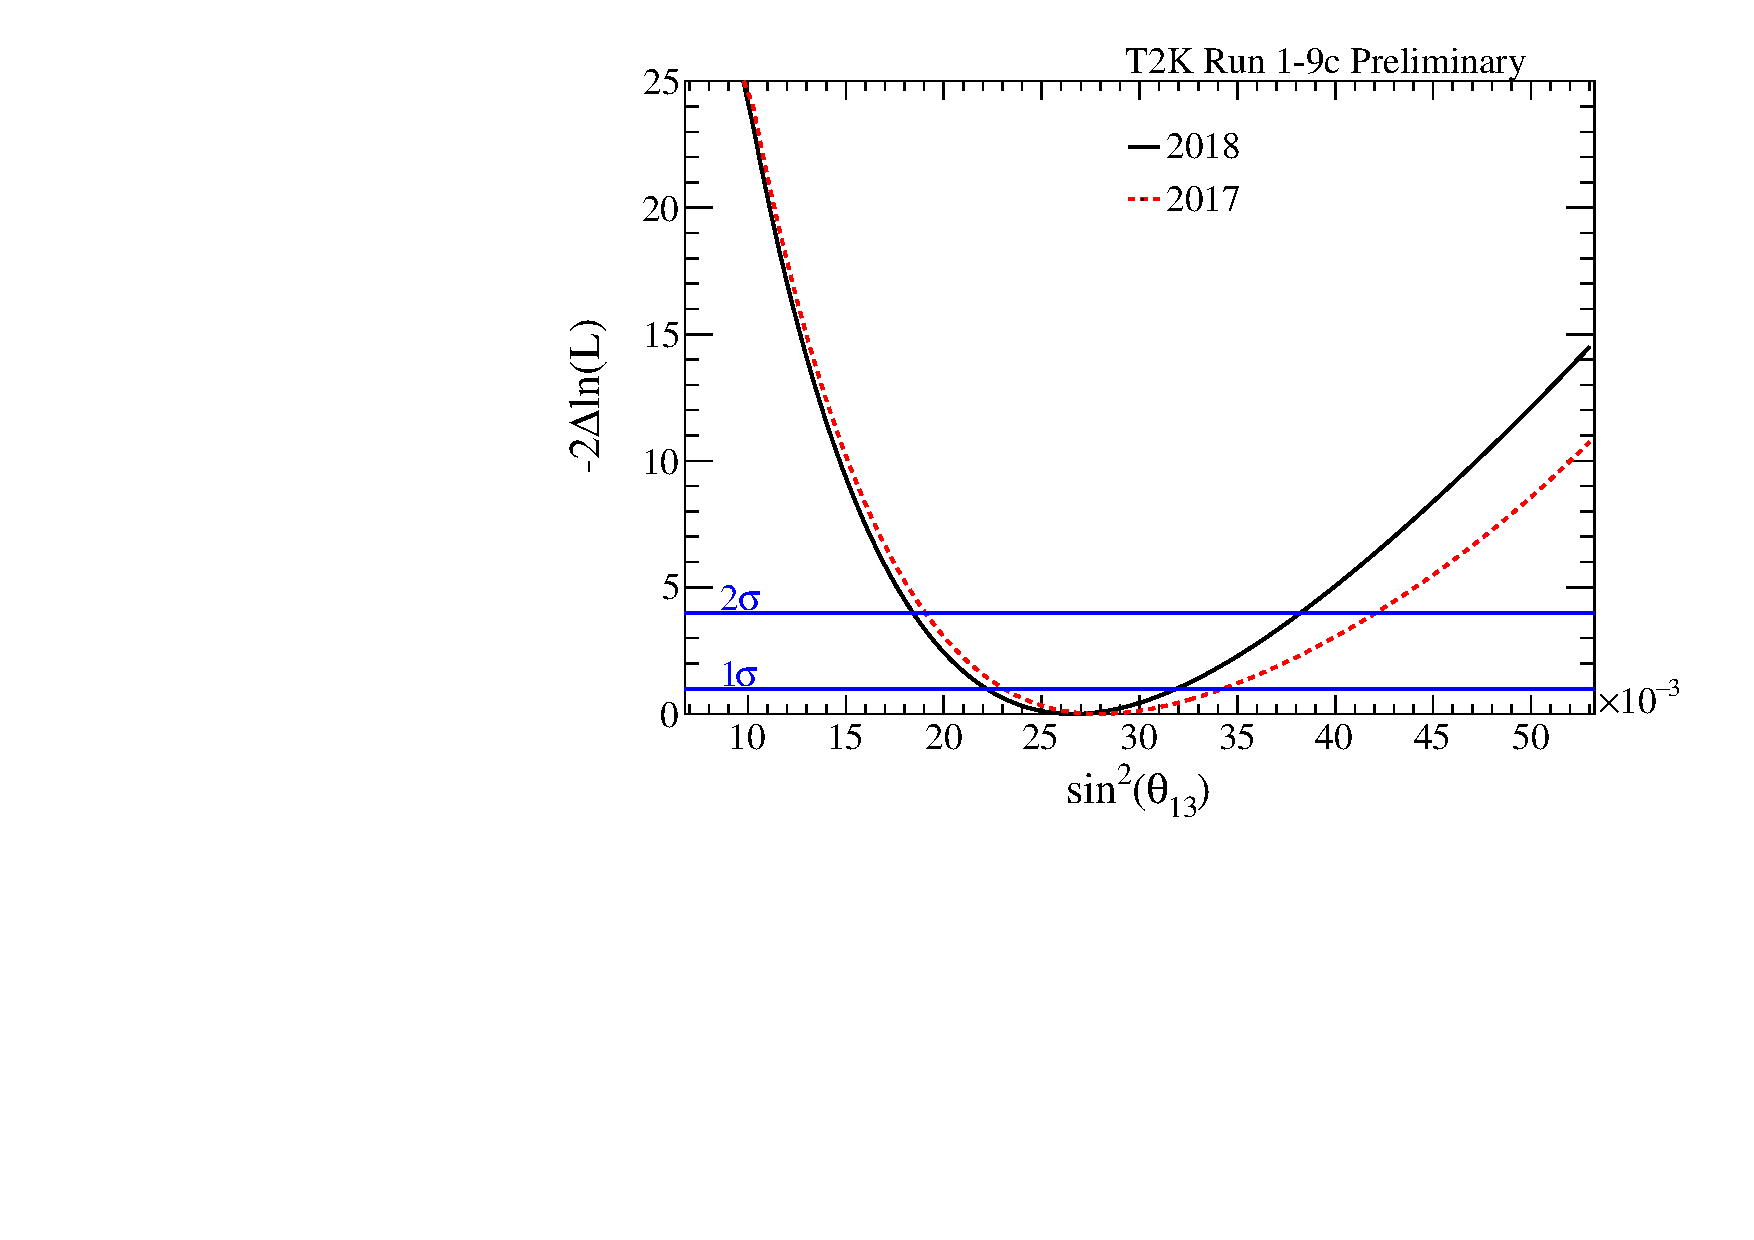
\includegraphics[width=0.9\textwidth]{images/data/comparison/theta13_worc_normal_2018_v_2017}
		\caption{\ssqthonethree NH without reactor constraint}
	\end{subfigure}
	\begin{subfigure}[b]{0.49\textwidth}
		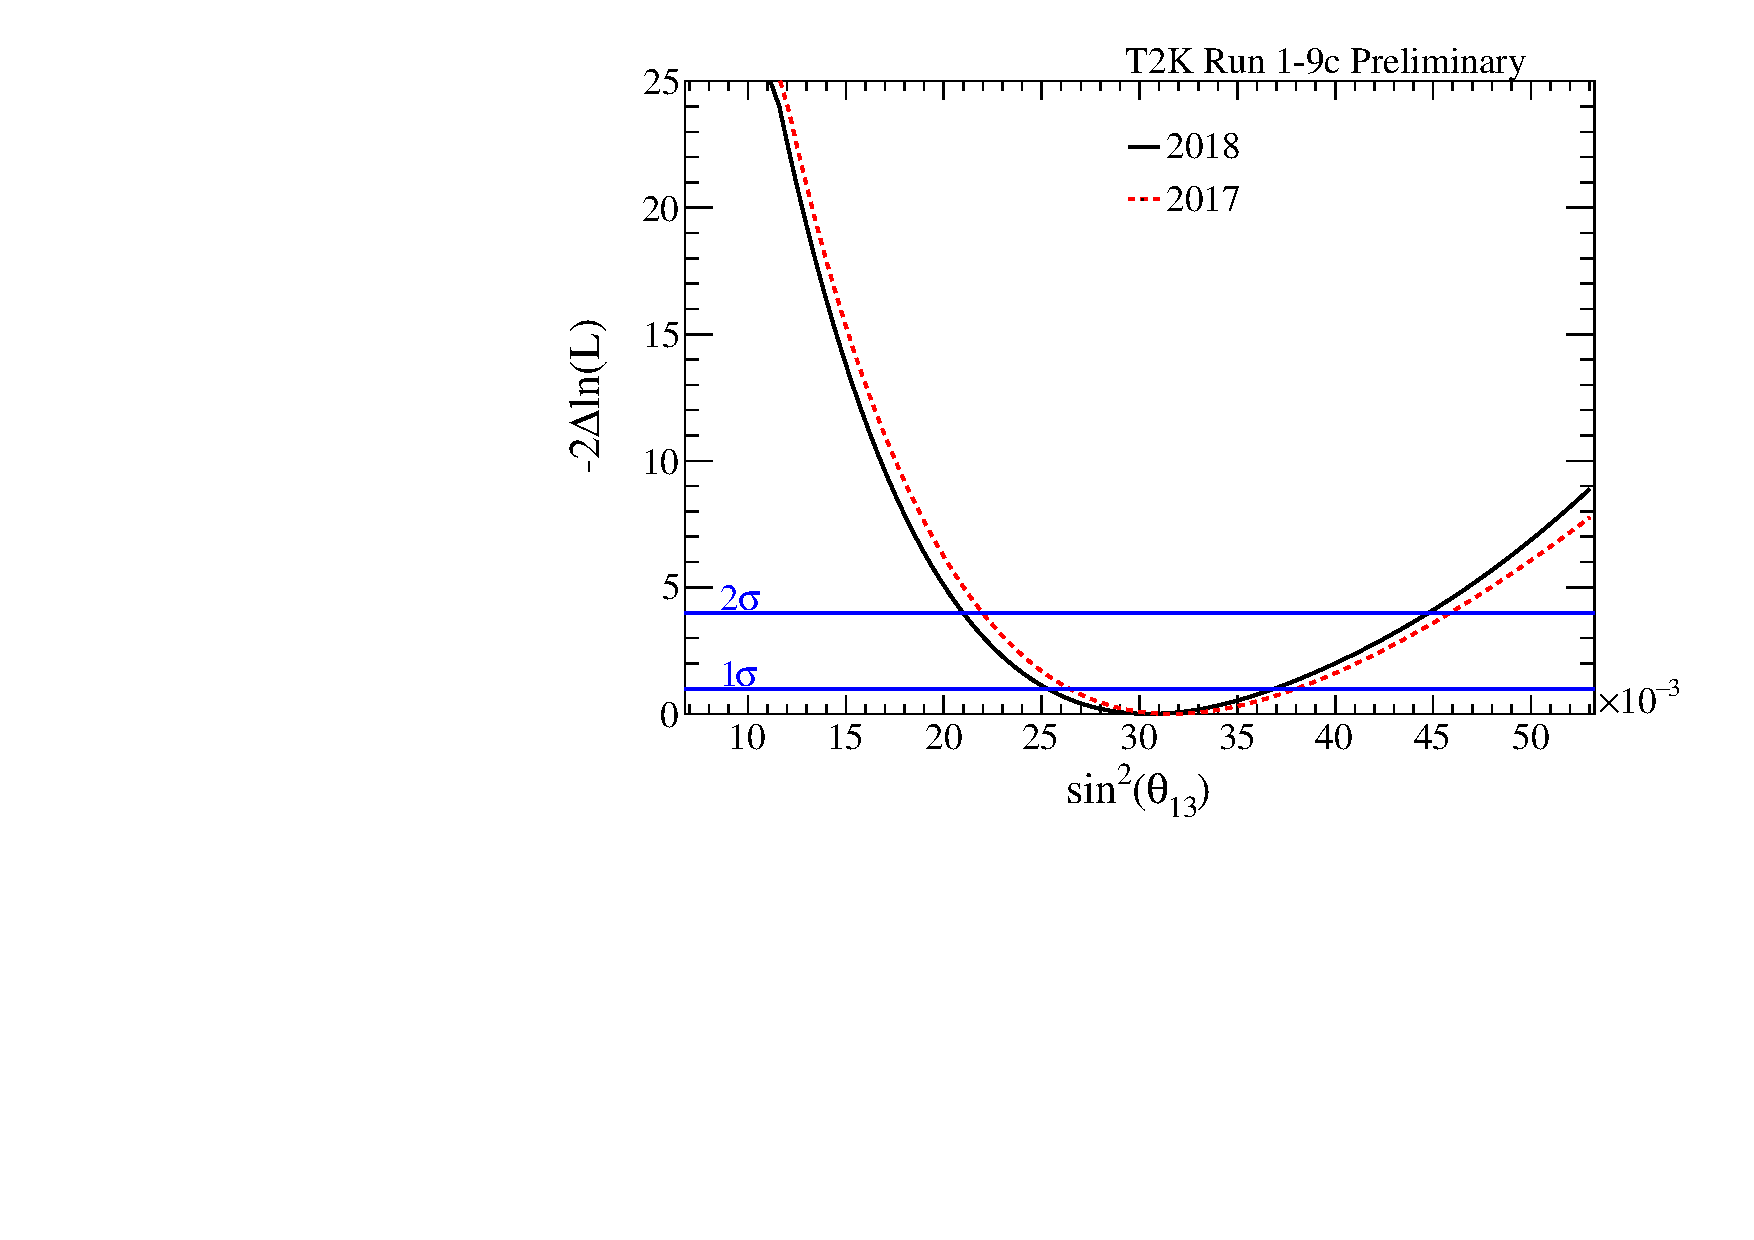
\includegraphics[width=0.9\textwidth]{images/data/comparison/theta13_worc_inverted_2018_v_2017}
		\caption{\ssqthonethree IH without reactor constraint}
	\end{subfigure}
	\caption {
		The expected $\Delta\chi^2$ distribution as a function of \ssqthonethree without reactor constraint. Normal and inverted hierarchy contours are independent. All 5 samples were used to produce these fits.
	}
	\label{fig:th13_data_compare}
\end{figure*}

\clearpage

\subsection{Results for \ssqthtwothree}

The result for \ssqthtwothree with reactor constraint and T2K only is shown in fig.~\ref{fig:th23_data_compare}. As noted for the appearance fit, the best-fit values for \ssqthtwothree have shifted away from maximal disappearance.

\begin{figure*}[htb]
	\center
	\begin{subfigure}[b]{0.49\textwidth}
		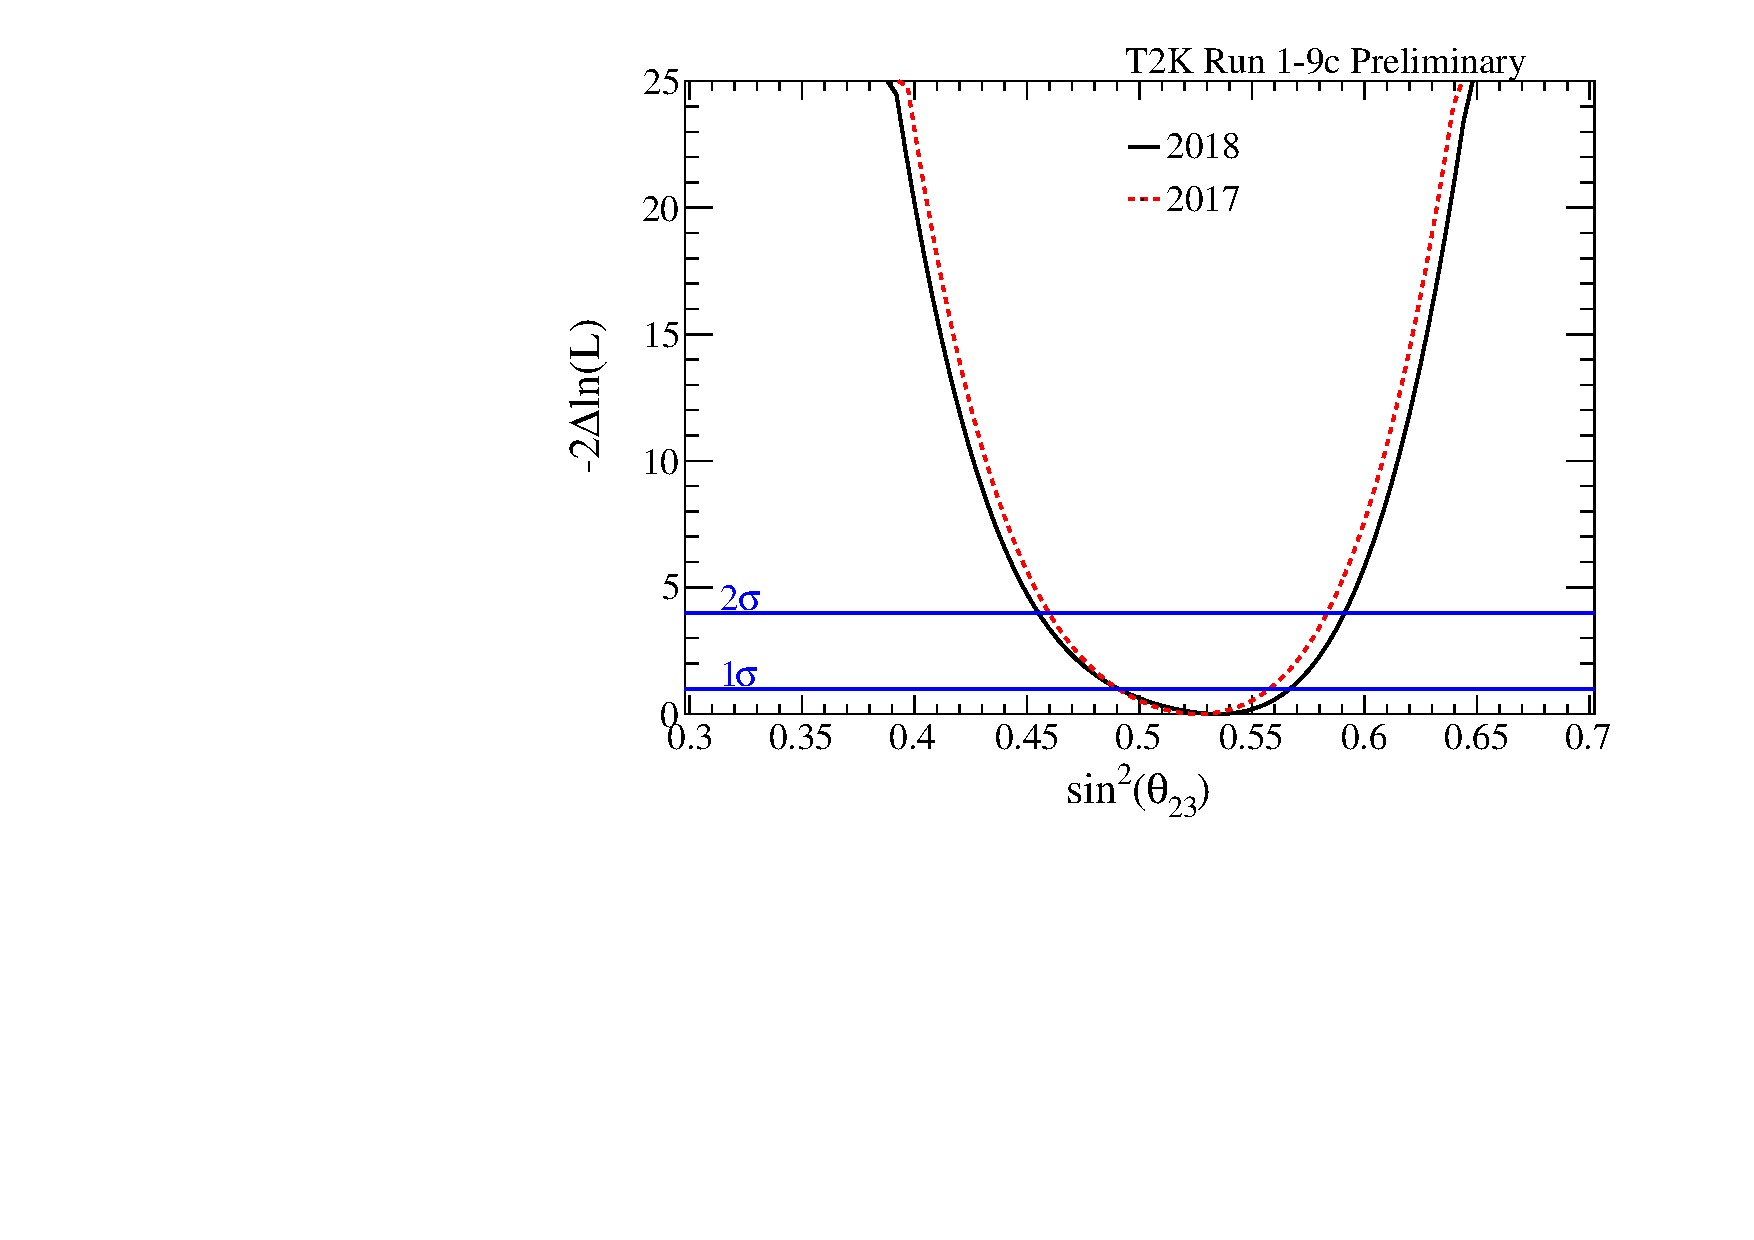
\includegraphics[width=0.9\textwidth]{images/data/comparison/theta23_wrc_normal_2018_v_2017}
		\caption{\ssqthtwothree NH with reactor constraint}
	\end{subfigure}
	\begin{subfigure}[b]{0.49\textwidth}
		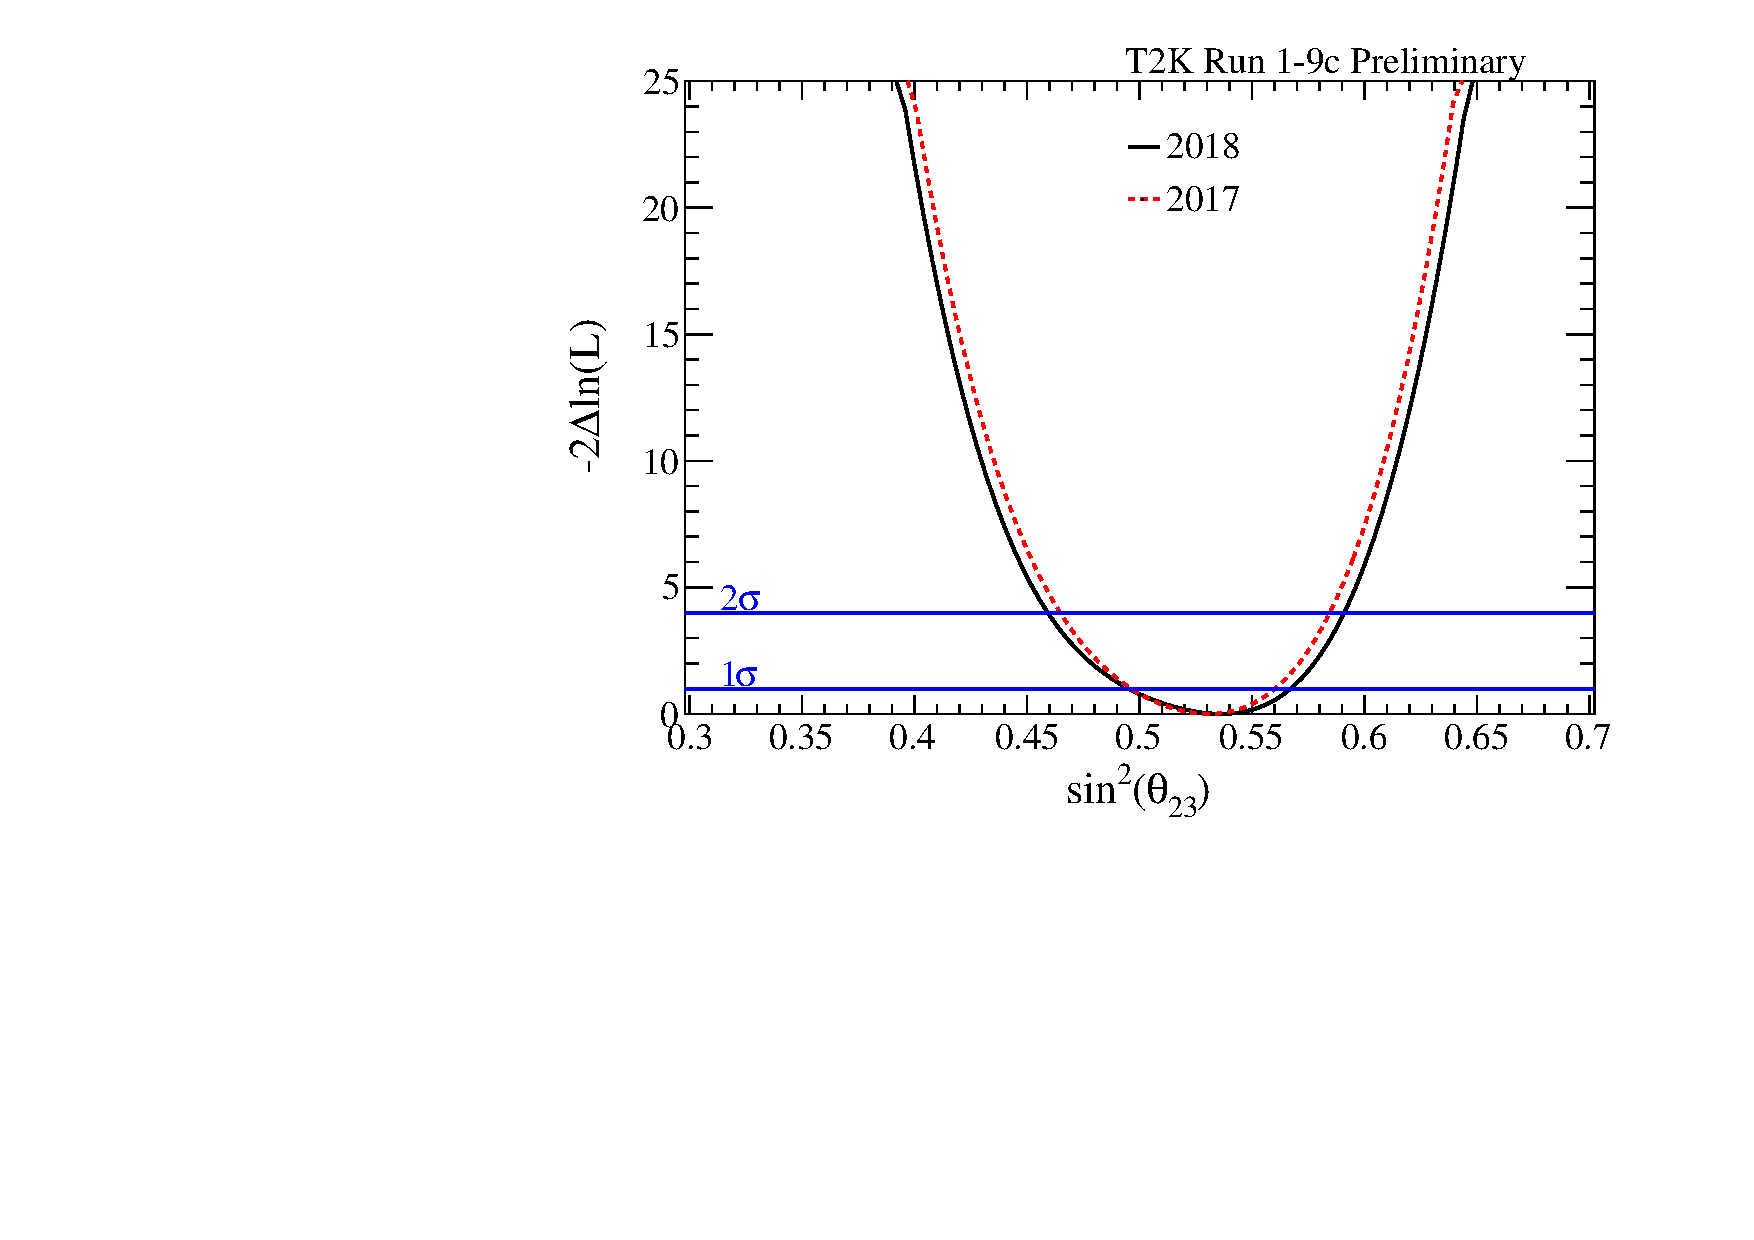
\includegraphics[width=0.9\textwidth]{images/data/comparison/theta23_wrc_inverted_2018_v_2017}
		\caption{\ssqthtwothree IH with reactor constraint}
	\end{subfigure}
	\begin{subfigure}[b]{0.49\textwidth}
		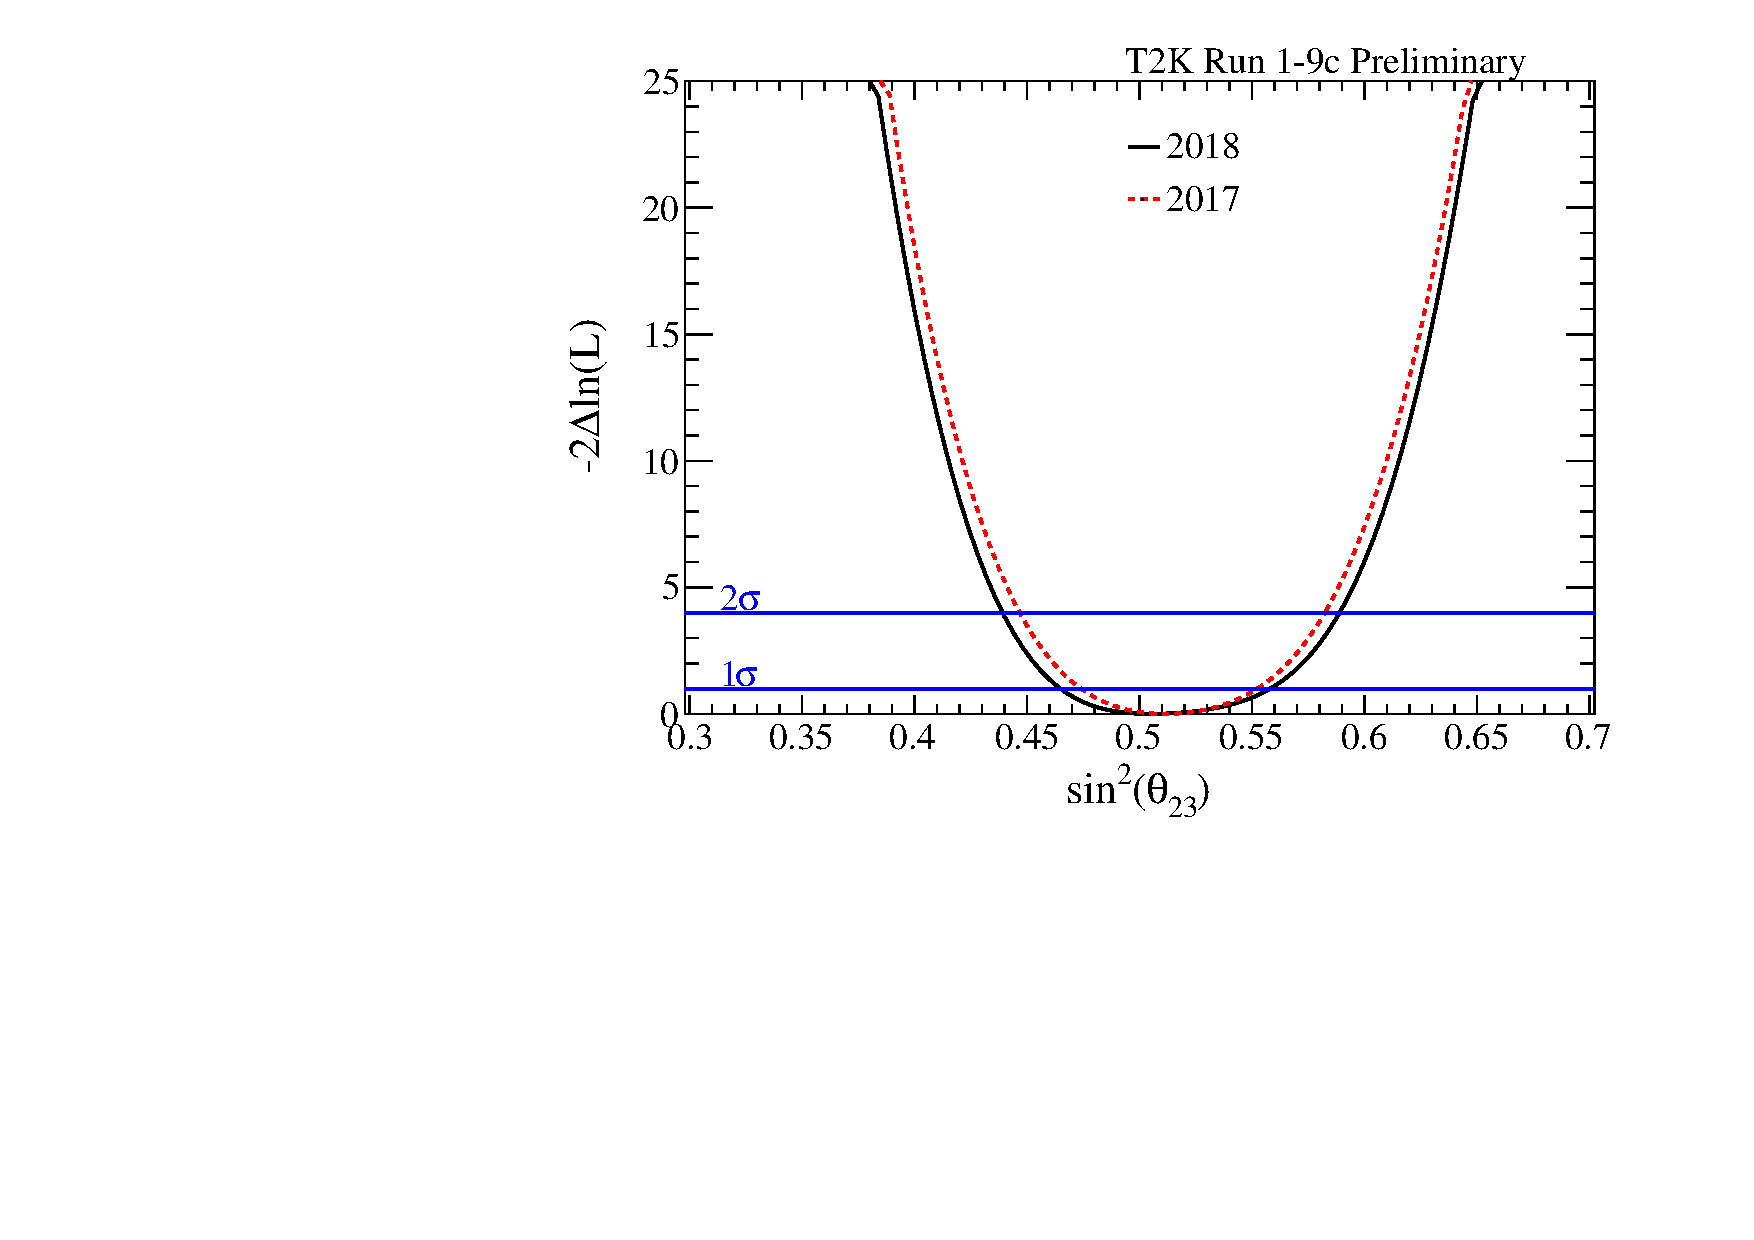
\includegraphics[width=0.9\textwidth]{images/data/comparison/theta23_worc_normal_2018_v_2017}
		\caption{\ssqthtwothree NH without reactor constraint}
	\end{subfigure}
	\begin{subfigure}[b]{0.49\textwidth}
		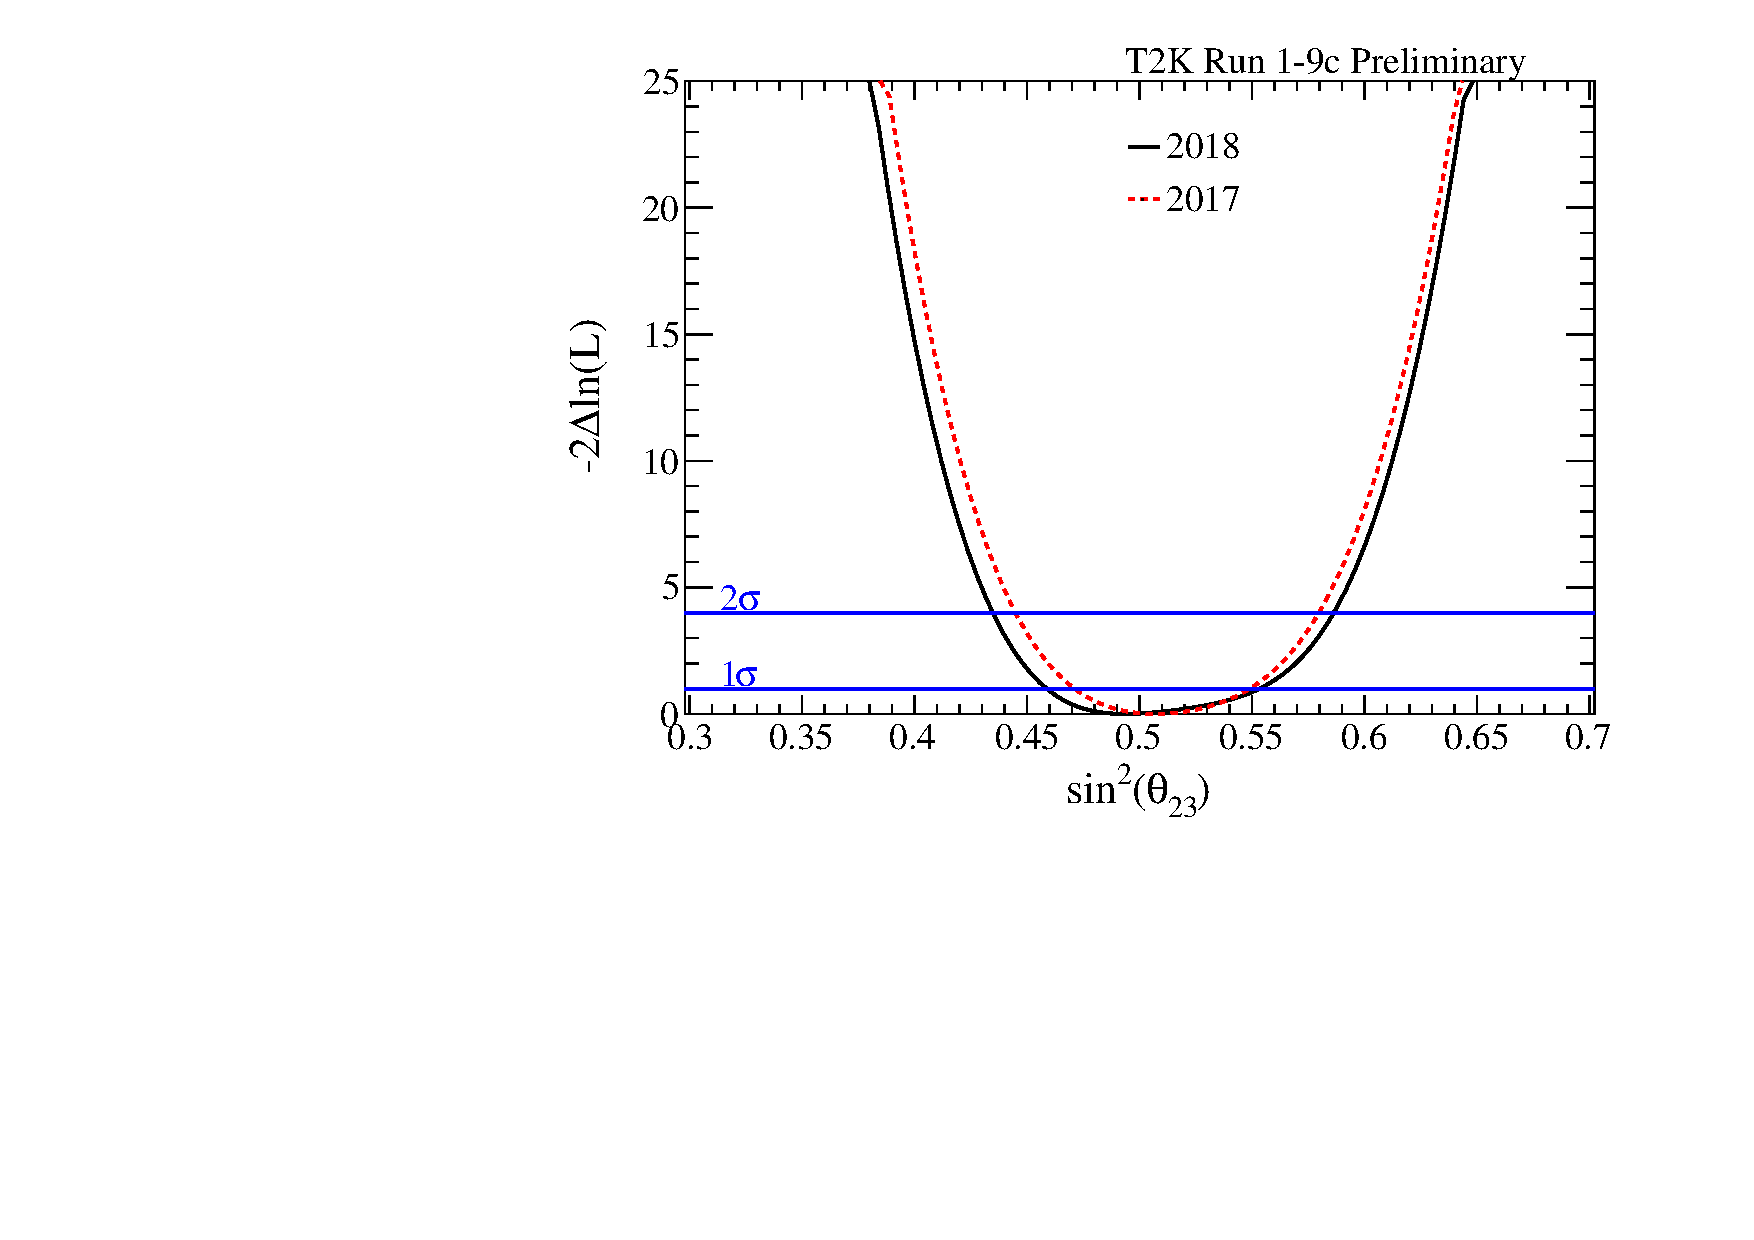
\includegraphics[width=0.9\textwidth]{images/data/comparison/theta23_worc_inverted_2018_v_2017}
		\caption{\ssqthtwothree IH without reactor constraint}
	\end{subfigure}
	\caption {
		The expected $\Delta\chi^2$ distribution as a function of \ssqthtwothree with and without reactor constraint. Normal and inverted hierarchy contours are independent. All 5 samples were used to produce these fits.
	}
	\label{fig:th23_data_compare}
\end{figure*}
\clearpage

\subsection{Results for \dmsq}

The result for \dmsq with reactor constraint and T2K only is shown in fig.~\ref{fig:dmsq_data_compare}. The \RunPeriod data favour lower values of \dmsq relative to \PrevRunPeriod, though the overall width of the contour is largely unchanged.

\begin{figure*}[htb]
	\center
	\begin{subfigure}[b]{0.49\textwidth}
		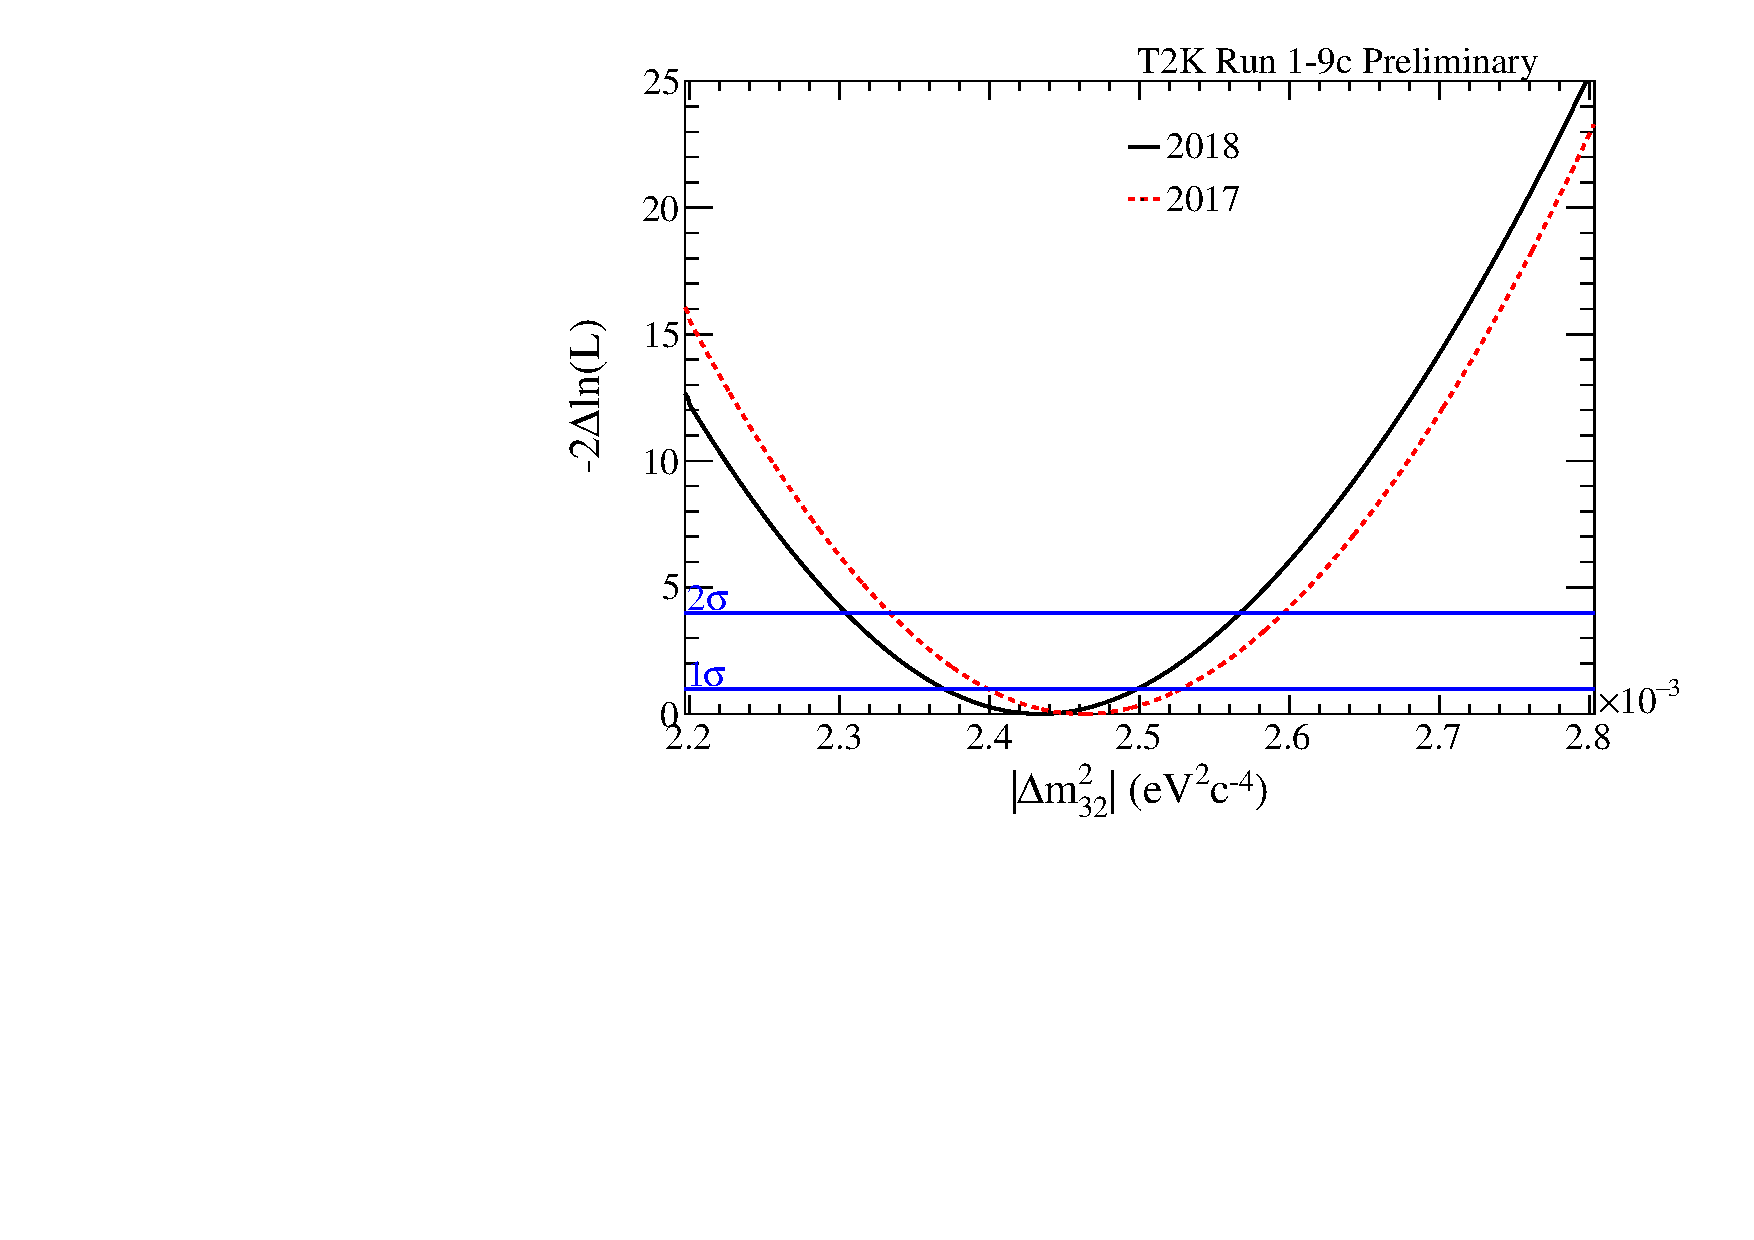
\includegraphics[width=0.9\textwidth]{images/data/comparison/dmsq_wrc_normal_2018_v_2017}
		\caption{\dmsq NH with reactor constraint}
	\end{subfigure}
	\begin{subfigure}[b]{0.49\textwidth}
		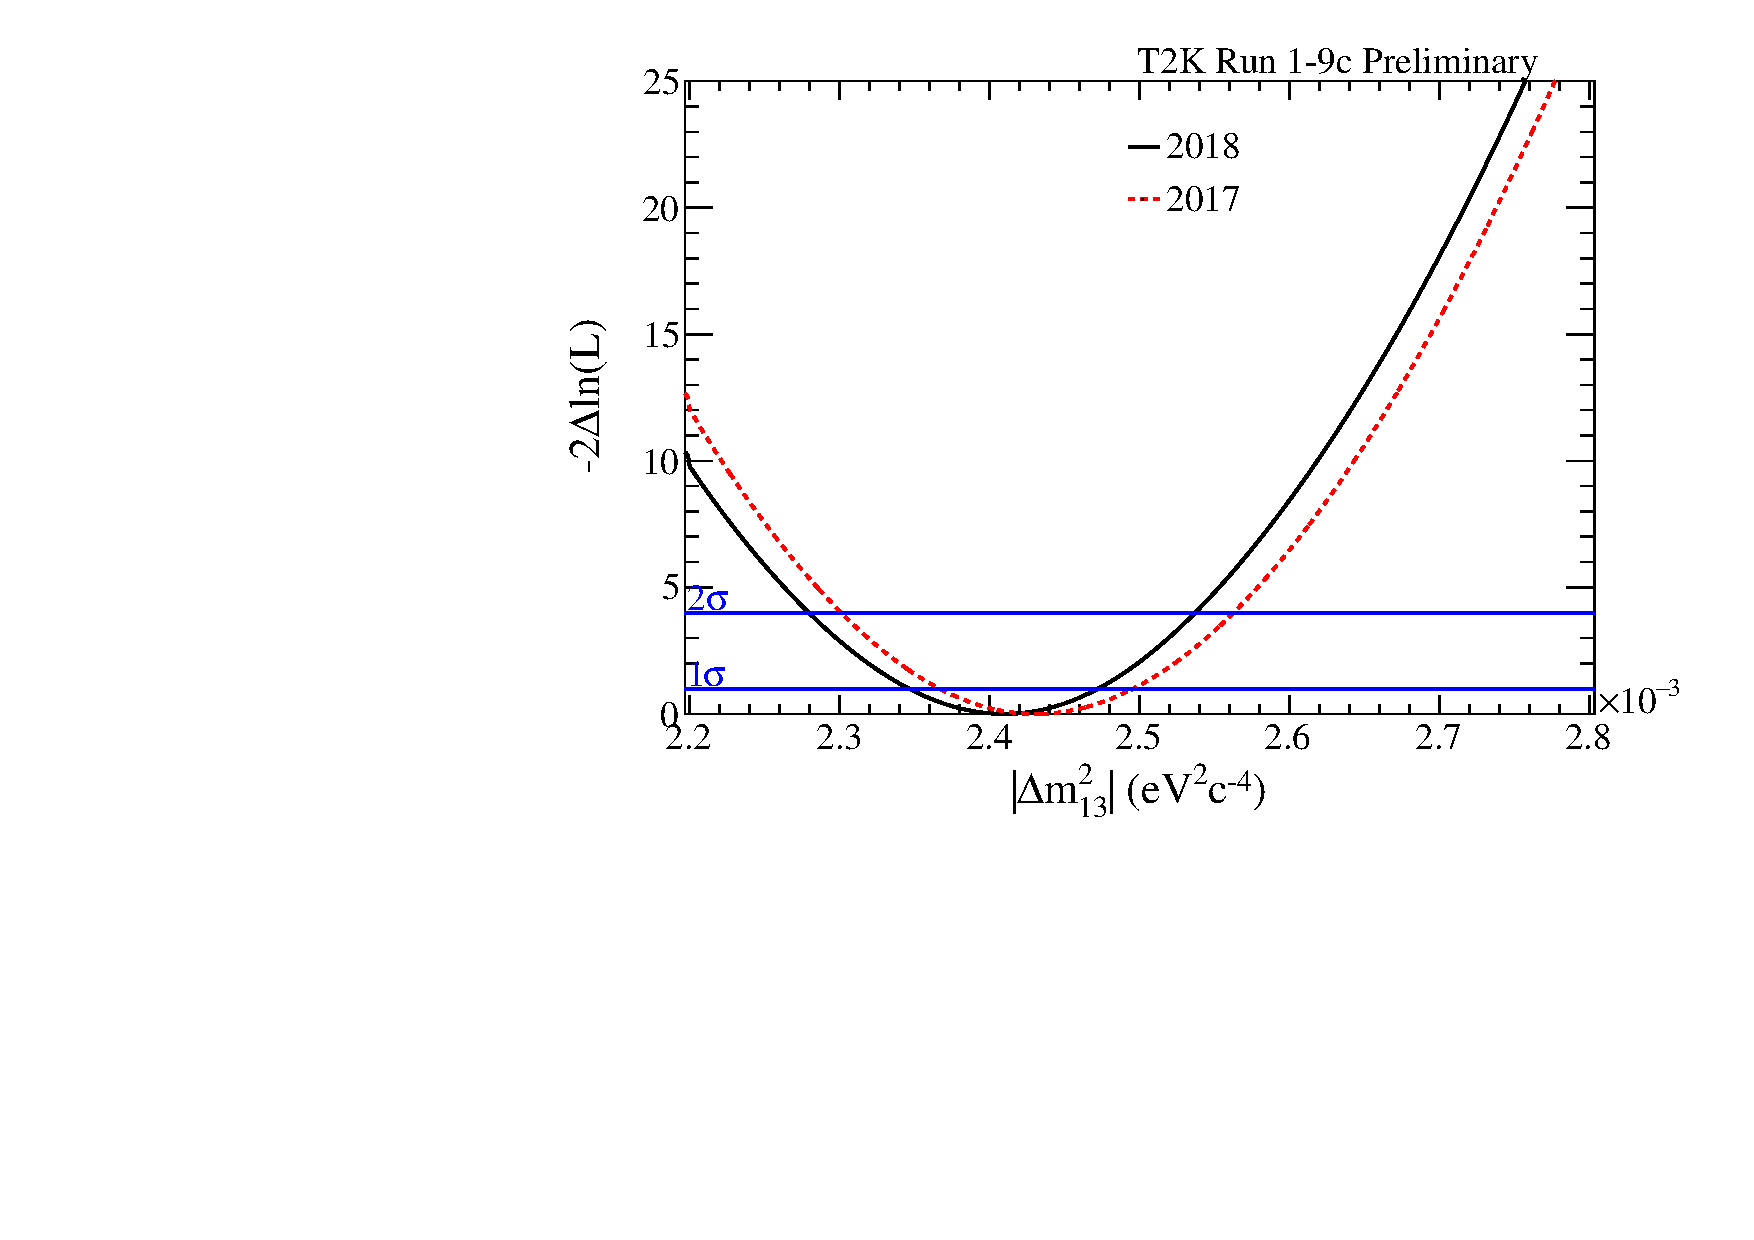
\includegraphics[width=0.9\textwidth]{images/data/comparison/dmsq_wrc_inverted_2018_v_2017}
		\caption{\dmsq IH with reactor constraint}
	\end{subfigure}
	\begin{subfigure}[b]{0.49\textwidth}
		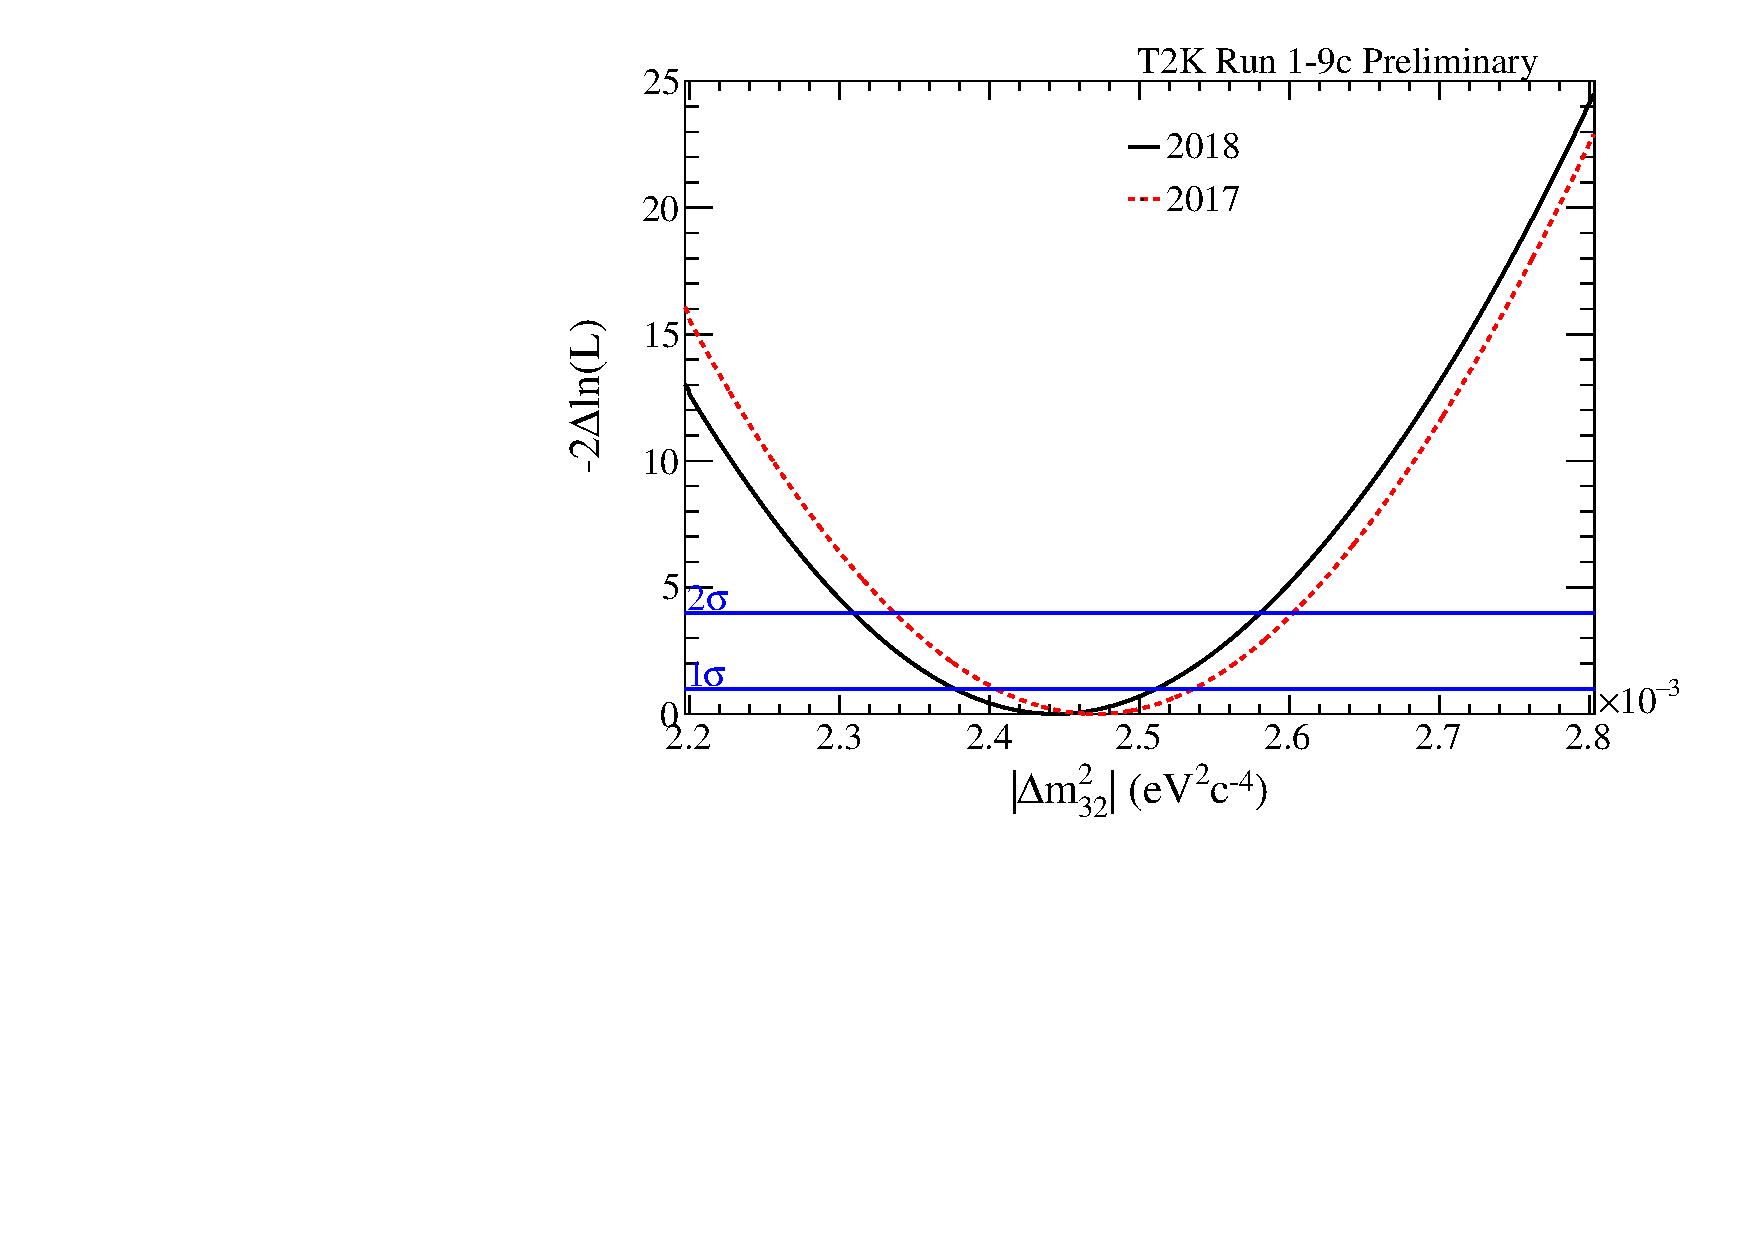
\includegraphics[width=0.9\textwidth]{images/data/comparison/dmsq_worc_normal_2018_v_2017}
		\caption{\dmsq NH without reactor constraint}
	\end{subfigure}
	\begin{subfigure}[b]{0.49\textwidth}
		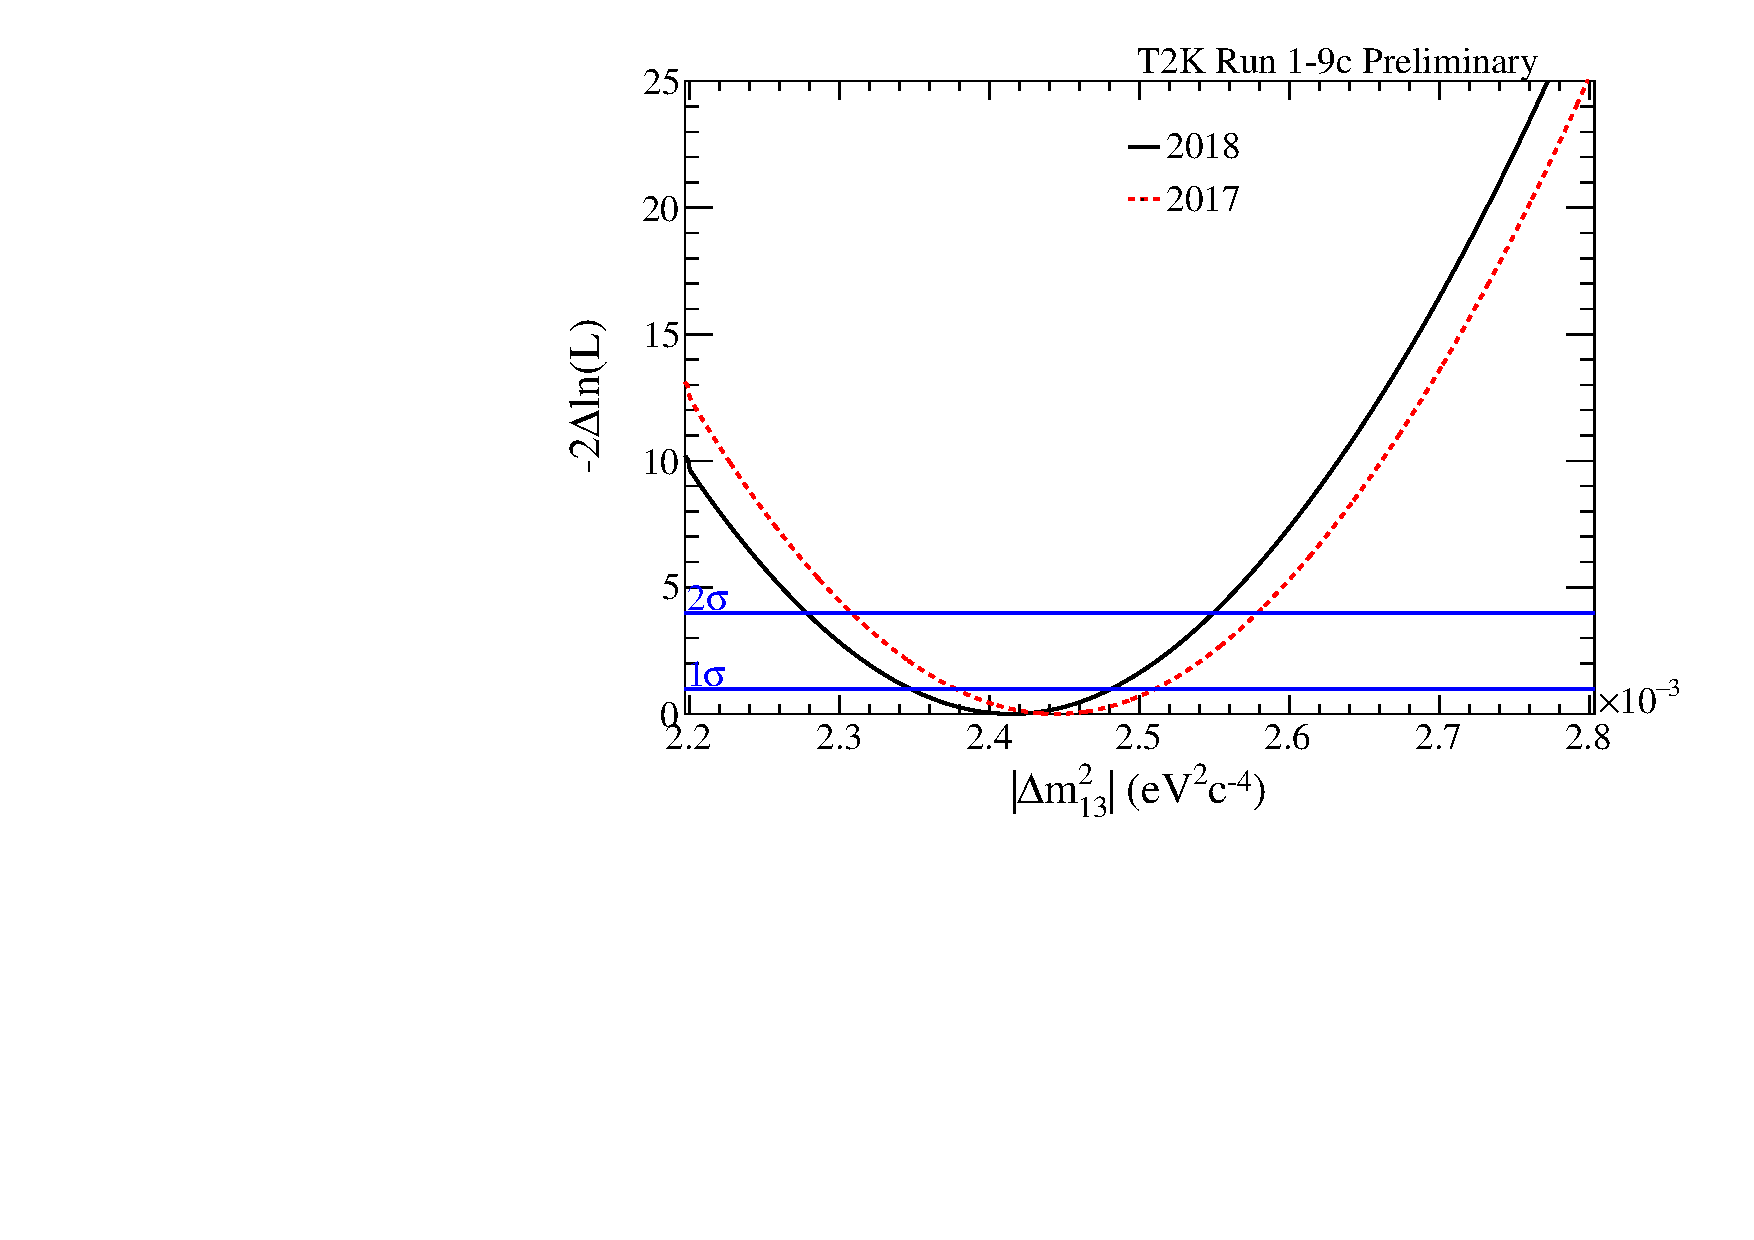
\includegraphics[width=0.9\textwidth]{images/data/comparison/dmsq_worc_inverted_2018_v_2017}
		\caption{\dmsq IH without reactor constraint}
	\end{subfigure}
	\caption {
		The expected $\Delta\chi^2$ distribution as a function of \dmsqtwothree with and without reactor constraint. Normal and inverted hierarchy contours are independent. All 5 samples were used to produce these fits.
	}
	\label{fig:dmsq_data_compare}
\end{figure*}

\clearpage